%%%%%%%%%%%%%%%%%%%%%%%%%%
%% nonofficial template %%
%%%%%%%%%%%%%%%%%%%%%%%%%%

\documentclass[12pt]{report}


%%%%%%%%%%%%%%%%%%%%%%%%%%
%% global configuration %%
%%%%%%%%%%%%%%%%%%%%%%%%%%

%%%%%%%%%%%%%%%%%%%%%%%%%%
%% global configuration %%
%%%%%%%%%%%%%%%%%%%%%%%%%%

%the overline configuration on the pages-----------
%mainly refer to "packages.tex" in https://www.overleaf.com/latex/templates/tesi-unitn/jjrxgvzgxpsm
\usepackage{fancyhdr}
\pagestyle{fancy}
\fancyhf{}
\fancyhead[LE]{\leftmark} %left page with leftmark of chapter
\fancyhead[RO]{\rightmark} %right page with rightmark of section
\fancyfoot[LE,RO]{\thepage} %the position of page number
%the overline configuration on the pages-----------
%--------------------------------------------------


%clear the empty double page-----------------------
%refer to https://texfaq.org/FAQ-reallyblank
\let\origdoublepage\cleardoublepage
\newcommand{\clearemptydoublepage}{%
    \clearpage{\pagestyle{empty}\origdoublepage}%
    }
\let\cleardoublepage\clearemptydoublepage
%clear the empty double page-----------------------
%--------------------------------------------------


%make the reference clickable----------------------
\usepackage{hyperref}
\hypersetup{  
    colorlinks=true, 
    linkcolor=black, 
    citecolor=red, 
    urlcolor=blue  
    }
%make the reference clickable----------------------
%--------------------------------------------------


%bibliography--------------------------------------
%refer to https://www.overleaf.com/learn/latex/Bibliography_management_in_LaTeX
\usepackage[
    backend=biber,
    style=alphabetic,
    sorting=ynt
    ]{biblatex}
\addbibresource{biblitex.bib} %Import the bibliography file
\usepackage{url} %make the online sites clickable
%bibliography--------------------------------------
%--------------------------------------------------


%colors&figures------------------------------------
\usepackage{geometry} % adjust the pages configuration
\usepackage{graphicx} % insert figures
\usepackage[export]{adjustbox} % for title page
\usepackage{xcolor}
\usepackage{float} %used to place figure with specifier [H]
%colors&figures------------------------------------
%--------------------------------------------------

\usepackage{lscape}
\usepackage[table,xcdraw]{xcolor}
\usepackage{graphicx}
%others--------------------------------------------
\usepackage{enumitem} % to use "description" environment
%others--------------------------------------------
%--------------------------------------------------



%%%%%%%%%%%%%%%%
%% title page %%
%%%%%%%%%%%%%%%%

%the watermark on the title page-------------------
%mainly refer to "ULBreport.cls" in https://it.overleaf.com/latex/templates/ulbreport-template/jzjgsqbnswmw
\usepackage[pages=some]{background} %"pages=some" is used to select pages for the background. If you need it for all pages, just delete "[pages=some].
\backgroundsetup{
    firstpage = true,
    scale=1,
    color=black,
    opacity=0.05,
    angle=0,
    position={6.3,-23.4},
    contents={
        
\includegraphics[
            height=20cm,
            width=20cm,
            keepaspectratio
            ]{picture/image1.png}
        }
    }
%the watermark on the title page-------------------
%--------------------------------------------------


%information settings------------------------------
%mainly refer to "document_settings.tex" in https://www.overleaf.com/latex/templates/hpi-phd-thesis-template/tggbwxzmzvkr

\newcommand{\printTitle}{}% The title of the thesis.
\newcommand{\myTitle}[1]{\renewcommand{\printTitle}{#1}}

\newcommand{\printAuthor}{}% The author’s name.
\newcommand{\myName}[1]{\renewcommand{\printAuthor}{#1}}

\newcommand{\printSupervisor}{}% The name of the author’s supervisor.
\newcommand{\mySupervisor}[1]{\renewcommand{\printSupervisor}{#1}}

\newcommand{\printAffSupervisor}{}% The affiliation of the supervisor.
\newcommand{\affSupervisor}[1]{\renewcommand{\printAffSupervisor}{#1}}

\newcommand{\printDate}{}% The date of the defense.
\newcommand{\myDate}[1]{\renewcommand{\printDate}{#1}}

\myTitle{Road Network Similarity Metrics}
\myName{Praise Ogunreku}
\mySupervisor{Prof.~Dr.-Ing.~Martin Kada}
\affSupervisor{Prof. Dr.-Ing. Roman Galas}
%information settings------------------------------
%--------------------------------------------------


%%%%%%%%%%%%%%%%%%%%%%%%%%%%%%%%%%%%%%%%%
% Math required package & abbreviations %
%%%%%%%%%%%%%%%%%%%%%%%%%%%%%%%%%%%%%%%%%

%%%%%%%%%%%%%%%%%%%%%%%%%%%%%%%%%%%%%%%%%%
% Math required packages & abbreviations %
%%%%%%%%%%%%%%%%%%%%%%%%%%%%%%%%%%%%%%%%%%

%list of symbols-----------------------------------
\usepackage{nomencl}
\renewcommand{\nomname}{List of Symbols}
%list of symbols-----------------------------------
%--------------------------------------------------


%math font-----------------------------------------
\usepackage{amsfonts}
\usepackage{amssymb}
\usepackage{amsmath}
\usepackage{bm} % bold letter in math mode 
\usepackage{mathrsfs} % decorated letter
\usepackage{bbm} % indicative function 1
\usepackage{extarrows} % http://ctan.org/pkg/extarrows
%math font-----------------------------------------
%--------------------------------------------------


%theories------------------------------------------
\usepackage{amsthm}

\newtheorem{theorem}{Theorem}[chapter]
\newtheorem{cor}{Corollary}[theorem]
\newtheorem{lemma}{Lemma}[chapter]
\newtheorem{remark}{Remark}[chapter]
\newtheorem{definition}{Definition}
\newtheorem{prop}{Proposition}[chapter]
\newtheorem{example}{Example}[chapter]

\numberwithin{equation}{section}
%theorems------------------------------------------
%--------------------------------------------------

%some abbreviations--------------------------------
\renewcommand{\a}{\alpha}
\renewcommand{\b}{\beta}

\renewcommand{\AA}{\mathbb{A}}
\newcommand{\BB}{\mathbb{B}}
\newcommand{\CC}{\mathbb{C}}
\newcommand{\DD}{\mathbb{D}}
\newcommand{\EE}{\mathbb{E}}
\newcommand{\FF}{\mathbb{F}}
\newcommand{\GG}{\mathbb{G}}
\newcommand{\HH}{\mathbb{H}}
\newcommand{\II}{\mathbb{I}}
\newcommand{\JJ}{\mathbb{J}}
\newcommand{\KK}{\mathbb{K}}
\newcommand{\LL}{\mathbb{L}}
\newcommand{\MM}{\mathbb{M}}
\newcommand{\NN}{\mathbb{N}}
\newcommand{\OO}{\mathbb{O}}
\newcommand{\PP}{\mathbb{P}}
\newcommand{\QQ}{\mathbb{Q}}
\newcommand{\RR}{\mathbb{R}}
\renewcommand{\SS}{\mathbb{S}}
\newcommand{\TT}{\mathbb{T}}
\newcommand{\UU}{\mathbb{U}}
\newcommand{\VV}{\mathbb{V}}
\newcommand{\WW}{\mathbb{W}}
\newcommand{\XX}{\mathbb{X}}
\newcommand{\YY}{\mathbb{Y}}
\newcommand{\ZZ}{\mathbb{Z}}

\newcommand{\mcA}{\mathcal{A}}
\newcommand{\mcB}{\mathcal{B}}
\newcommand{\mcC}{\mathcal{C}}
\newcommand{\mcD}{\mathcal{D}}
\newcommand{\mcE}{\mathcal{E}}
\newcommand{\mcF}{\mathcal{F}}
\newcommand{\mcG}{\mathcal{G}}
\newcommand{\mcH}{\mathcal{H}}
\newcommand{\mcI}{\mathcal{I}}
\newcommand{\mcJ}{\mathcal{J}}
\newcommand{\mcK}{\mathcal{K}}
\newcommand{\mcL}{\mathcal{L}}
\newcommand{\mcM}{\mathcal{M}}
\newcommand{\mcN}{\mathcal{N}}
\newcommand{\mcO}{\mathcal{O}}
\newcommand{\mcP}{\mathcal{P}}
\newcommand{\mcQ}{\mathcal{Q}}
\newcommand{\mcR}{\mathcal{R}}
\newcommand{\mcS}{\mathcal{S}}
\newcommand{\mcT}{\mathcal{T}}
\newcommand{\mcU}{\mathcal{U}}
\newcommand{\mcV}{\mathcal{V}}
\newcommand{\mcW}{\mathcal{W}}
\newcommand{\mcX}{\mathcal{X}}
\newcommand{\mcY}{\mathcal{Y}}
\newcommand{\mcZ}{\mathcal{Z}}

\newcommand{\mfa}{\mathfrak{a}}
\newcommand{\mfb}{\mathfrak{b}}
\newcommand{\mfc}{\mathfrak{c}}
\newcommand{\mfp}{\mathfrak{p}}
\newcommand{\mfq}{\mathfrak{q}}

% with high frequency

\newcommand{\indi}[1]{\mathbbm{1}_{#1}} % indicative function 1
\renewcommand{\l}{\langle} % < bra
\renewcommand{\r}{\rangle} % > ket
\newcommand{\bk}[2]{\langle#1, #2\rangle} % <,> bracket, inner prod
\renewcommand{\d}{\differential}
\newcommand{\supp}[1]{\operatorname{supp}(#1)}
\newcommand{\Id}{\operatorname{Id}}
\newcommand{\p}[1]{\partial_{#1}}
\newcommand{\LR}[1]{\left(#1\right)} % auto ( )
\newcommand{\red}[1]{{\color{red}(#1)}} %red notation
\newcommand{\half}{\frac{1}{2}} % 0.5, 1/2

%Prob

\newcommand{\EEE}[1]{\mathbb{E}\left[#1\right]}
\newcommand{\PPP}[1]{\mathbb{P}\left(#1\right)}
\newcommand{\Cov}[2]{\operatorname{Cov}(#1,#2)}
\newcommand{\prc}[2]{(#1)_{#2\in\RR^+}}
\newcommand{\seq}[2]{(#1)_{#2\in\NN}}

%topology

\newcommand{\Int}{\operatorname{Int}}
\newcommand{\dist}[2]{\operatorname{d}(#1,#2)}

%algebra

\newcommand{\ord}[1]{\operatorname{order}\left(#1\right)}
\newcommand{\Vect}{\operatorname{Vect}}
\newcommand{\Hom}[2]{\operatorname{Hom}(#1,#2)}
\newcommand{\gcdt}[2]{\operatorname{gcd}(#1,#2)}
\newcommand{\lcm}[2]{\operatorname{lcm}(#1,#2)}
%some abbreviations--------------------------------
%--------------------------------------------------



%%%%%%%%%%%%%%%%%%%%%%%%%%%%%%%%%%%%%%%%%%%%%%%%%%%
%~~~~~~~~~~~~~~~~~~~~~~~~~~~~~~~~~~~~~~~~~~~~~~~~~%
%%%%%%%%%%%%%%%%%%%%%%%%%%%%%%%%%%%%%%%%%%%%%%%%%%%


\begin{document}



%%%%%%%%%%%%%%%%
%% title page %%
%%%%%%%%%%%%%%%%

%covering------------------------------------------
%mainly refer to "title_page.tex" in https://www.overleaf.com/latex/templates/hpi-phd-thesis-template/tggbwxzmzvkr

\newgeometry{
    textwidth = 134 mm,
    textheight = 220 mm,
    left = 30 mm,
    right = 30 mm,
    }
    
\begin{titlepage}
    \begin{center}
        
\includegraphics[width=.25\textwidth,right]{picture/image1.png}
            \\
        \vspace*{0.8cm}
        {\Huge %title
            \rule[1 ex]{\textwidth}{2 pt} %upper line for the title
            \textbf{\printTitle}\\
            \rule[-1 ex]{\textwidth}{2 pt} %lower line for the title
            }
        \vfil
        {\Large Author:} \\[0.5cm]
        { %if there are more then one authors, just copy it in needed and add the corresponding newcommand in main.tex
            {\Large \textbf{\printAuthor}} \\[0.2cm]
            }
        \vfil
        {\Large Supervisor: }\\ [0.5cm]
        { %if there are more then one supervisors, just copy it in needed and add the corresponding newcommand in main.tex
            {\Large \textbf{\printSupervisor}} \\[0.2cm]
            }
        \vfil
        {Fakult\"at IV - Planning, Building, Environment \\Institute of Geodesy and Geoinformation Science  \\ Technischen Universit\"at Berlin } \\[2 pt]
        \vfil
        {A thesis submitted in fulfillment of the requirements for the degree of \\ Master of Science in Geodesy and Geoinformation Science}
        \vfil
        {\large\textbf{30.03.2022} \printDate}
    \end{center}
\end{titlepage}

\restoregeometry
%covering------------------------------------------
%--------------------------------------------------


%the backside of covering--------------------------
%mainly refer to "ch0-backside.tex" in https://www.overleaf.com/latex/templates/unofficial-la-trobe-university-template/zfbdwvyrxshz
\hfill
\vfill

\noindent \textit{\printTitle} 
%{\textcopyright} {\printDate} 

\bigskip

\noindent Author:\\
{\printAuthor}

\medskip

\noindent Supervisor: \\
{\printSupervisor}
 % title page covering

\chapter*{Declaration}
    %%%%%%%%%%%%%%%
% Declaration %
%%%%%%%%%%%%%%%

I hereby declare that the thesis submitted is my own, unaided work, completed without any unpermitted external help. Only the sources and resources listed were used.


\vspace*{4em}\noindent
\hfill%
\begin{tabular}[t]{c}
  \rule{10em}{0.4pt}\\ Praise Ogunreku
\end{tabular}%
\hfill%
\begin{tabular}[t]{c}
  \rule{10em}{0.4pt}\\ Place, Date
\end{tabular}%
\hfill\strut


\chapter*{Zusammenfassung}
    %%%%%%%%%%%%
% Zusammenfassung %
%%%%%%%%%%%%

Das Verständnis der Ähnlichkeiten von Straßennetzstrukturen in Städten ist eine schwierige, aber notwendige Aufgabe für die Gestaltung besserer städtischer Umgebungen. Die Entdeckung und der Vergleich von Strukturen wie Graphen, modularen Gemeinschaften, reichen Clubs, Knotenpunkten und Bäumen liefern Informationen über die räumlichen und zeitlichen Eigenschaften von Straßennetzen.

Mit den jüngsten Fortschritten in der GIS- und Graphentheorie, der schnellen Zunahme verfügbarer Daten und der Flexibilität der Netzwerkmodellierung ist die Herausforderung entstanden, effiziente quantitative und garantierte Leistungsprioritäten zum Vergleichen von Straßennetzwerken zu entwickeln. Für diese Aufgabe gibt es viele Metriken, von denen die meisten in verschiedenen Bereichen wie Bioinformatik, Cybersicherheit und Analyse sozialer Netzwerke angewendet werden. Es wurde jedoch noch keine vergleichende Studie durchgeführt, um die Wirksamkeit dieser Metriken bei der Unterscheidung gängiger Straßennetztopologien auf verschiedenen strukturellen Maßstäben zu bestimmen.

Das Ziel dieses Papiers ist es, die am häufigsten verwendeten Entfernungsmetriken und -maße zu untersuchen und zu vergleichen und ihre Fähigkeit zu bewerten, zwischen topologischen Merkmalen in Straßennetzen zu unterscheiden. Schließlich werden die Metriken auf einen neuen spezialisierten Datensatz angewendet, der aus grafischen Darstellungen von Straßennetzen in 22 Städten besteht. Um die Ergebnisse dieser Art von Analyse zu diskutieren, enthalten die Datensätze eine Reihe leicht identifizierbarer Straßennetzmodelle.

Die experimentellen Ergebnisse zeigen, dass der in dieser Studie gewählte Ansatz nicht nur eine praktische Methode zur Identifizierung von Ähnlichkeiten in verschiedenen grafisch dargestellten Straßennetzen basierend auf ihren topologischen Merkmalen darstellt, sondern auch Ähnlichkeiten und Korrelationen im Verhalten der zur Identifizierung von Ähnlichkeiten verwendeten Metriken aufzeigt. in Straßennetzen eingesetzt.


\chapter*{Abstract}
    %%%%%%%%%%%%
% Abstract %
%%%%%%%%%%%%

Understanding the similarities of city road network structures is a difficult but necessary task for designing better urban environments. The discovery and comparison of structures such as graphs, modular communities, rich clubs, hubs, and trees provide information about the spatial and temporal properties of road networks.

With recent advancements in GIS and graph theory, and the rapid growth of available data and the flexibility of network modeling, the problem of developing effective quantitative and guaranteed a-priori notions of metrics for comparing road networks has arisen. Numerous metrics exist to accomplish this task, the majority of which are applied to various fields, including bioinformatics, cyber security, and social network analysis. However, no comparative study has been conducted to determine the efficacy of these metrics in distinguishing common road network topologies at various structural scales.

The purpose of this thesis is to explore and compare the most frequently used metrics and distance measures, and assess their ability to distinguish between common topological features found in road networks. Finally, the metrics are applied to a novel specialized data set consisting of graph representations of road networks in twenty-two cities. To discuss the results of this type of analysis, the data sets contain a collection of easily identifiable road network patterns.

Experimental results demonstrate that the approach adopted in this study not only provides a practical method of identifying similarities in different road networks represented as graphs based on their topological characteristics, but it also identifies similarities and correlations in the behavior of the metrics that are used to identify the similarities in the road networks.


    
\chapter*{Acknowledgements}
    %%%%%%%%%%%%%%%%%%%%
% Acknowledgements %
%%%%%%%%%%%%%%%%%%%%

I want to convey my heartfelt gratitude to my Supervisor, Prof Martin Kada, whose genuineness and encouragement I will never forget. Prof Kada has been an inspiration to me while I struggled through this Master's degree program. Furthermore, this thesis would not have been feasible without Amgad Agoub's supervision from the beginning of the research process, which allowed me to gain knowledge of the subject. I am grateful for the fantastic experiences he planned for me and the possibilities he provided for me to advance professionally. It is a privilege to learn from Prof. Martin Kada and Amgad Agoub.

I'd also want to thank my colleagues, Olumile Omole and Hassan El Hajj, for their effective feedback and programming suggestions during this project.

I am grateful to my parents, whose unwavering love and support keep me motivated and confident. My triumphs and success are the results of their faith in me. My heartfelt gratitude goes to my siblings, who keep me grounded, remind me of what is important in life, and always support my endeavors.

Finally, I want to express my heartfelt appreciation to Anita, my wife. I will be eternally grateful for the unending love and support I received daily throughout the thesis process.


\tableofcontents
\listoffigures
\listoftables

\chapter{Introduction}
    %%%%%%%%%%%%%%%%
% Introduction %
%%%%%%%%%%%%%%%%

The emerging geographic information system (GIS) repositories, such as EarthExplorer or OpenStreetMap (OSM), provide publicly accessible high-quality road network data and cadastre data that can be used to feed example-based urban modeling techniques with almost infinite examples. However, recognizing the similarities of patterns between the designs of several urban layouts remains a difficult job, even with a large amount of high-quality example data at hand. The key explanations are;  there are no guaranteed a-priori notion of metrics that can recognize the similar patterns in road networks and quantify the input of a given consumer into a realistic city layout that includes road networks.  Current modeling tools-sets have a steep learning curve and will require special education skills to work with them productively. Current automated methods rely on a set of rules and grammar to generate urban structures; however, their expressiveness is constrained by the collection of rules. Expert skills are required to effectively define the typeset rules and, in many cases, new rules-sets need to be developed for each new road network style created. In order to make it possible for non-expert users to create urban structures for individual experiments, this thesis proposes a portfolio of novel example-based metrics for managed evaluation of similar road networks for urban environments. The notion example-based implies that new virtual urban environments are generated by computer programs that re-use existing digitized real-world data that serve as models. The data, i.e., road networks, required to realize the envisioned task, are publicly accessible via online services. In order to enable the reuse of existing urban datasets, it is important to establish quantitative and qualitative metrics that encapsulate expert knowledge and thus enable the controlled evaluation of the similarity between different road network patterns.  

The focus of this thesis is to compare the similarity of various road network patterns in 21 major cities around the world using OpenStreetMap data. It proposes a series of a priori notions of available metrics in the literature that encapsulate the qualitative and quantitative characteristics required for the evaluation of the similarities between road networks as one of the fundamental structures common to urban environments and the best measure of similarity (a real number between 0 and 1) that captures the similarity of the two road networks as graphs well. Similarity measures are used to investigate the similarities and differences between these study sites across multiple dimensions.

The rest of this thesis is organized as follows: Chapter 2 briefly will provide the background on urban forms, past and current techniques for the detection of road network patterns, the basics of graph structure for representing road networks, and existing metrics used in literature for identifying similarities in graph networks. Chapter 3 discusses the data used in this approach  and presents the methodology of the thesis. Chapter 4 describes the results of the employed methodology on the data. Finally, chapter 5 presents Conclusion and recommendation for future work. 




\chapter{Related Work and Background}
    %%%%%%%%%%%%%%%
% Related Work and Background %
%%%%%%%%%%%%%%%

\section{Typology of Urban Forms}
To best understand the concept of road network patterns, one has to consider the urban forms of cities that best shape the road network patterns within such cities. Based on the literature on historic and more recent urban forms (for example, [\cite{deKlerk:1980} \& \cite{Rottier:1980}], identified six different forms (figure \ref{fig:urban forms})).
\begin{figure}[h]
\centering
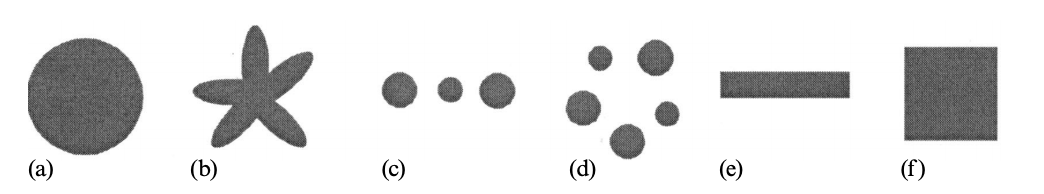
\includegraphics[width=0.95\textwidth,center]{picture/figure1.png}
\caption[Morphological Urban Forms]{Morphological urban forms: (a) the concentric city, (b) the lobe city, (c) the linear polynuclear city, (d) the concentric polynuclear city, (e) the linear city, (f) and the grid city.  Source: \cite{deKlerk:1980} \& \cite{Rottier:1980}}
\label{fig:urban forms}
\end{figure}

The concentric city represents the typical form of a city that has grown from a small (historic) center along a number of radial exit roads. Over the years the areas between the radial roads have been filled and the city has received its concentric form. This city shape is often associated with a radial road network, based on the historic routes, but combinations with ring or grid networks also exist. Often these cities are quite compact and have a strong center with a mixed supply of facilities.

The lobe city often has a similar history. The main differences are that the city has developed between some radial roads and not between others. The lobe shape can result from roads stretching out in some directions or from intentional city planning.

The linear polynuclear and concentric polynuclear cities have a number of things in common. The morphologies of these cities can develop in two very different ways. Either a number of smaller settlements, located close to each other, start to function as one city, or a city is actually designed as a polynuclear city. The only example of a true polynuclear city in the Netherlands is Almere, which can best be described as a concentric polynuclear city. 

The linear city can be viewed as an extreme version of the city form. These cities often have a grid-type transportation network for the car, but this is not necessarily the case. 

Grid cities is the collective noun for cities with a more or less rectangular shape. In the selection of locations for data collection these four types (concentric city, lobe city, and grid city) were included.

\section{Road network patterns}
The complexities of shape and structure set road patterns apart from many other objects of urban or transport analysis. For example, road width is merely a linear quantity and traffic flow is a simple ratio (vehicles per hour). Even the issue of density boils down to a straightforward ratio, however fiercely the significance of different numerators or denominators may be contested. By contrast, there is no straightforward or standard descriptor that is used to capture road patterns. 

Yet, unless we have an adequate description of pattern or structure, it will remain difficult to compare structures across cases – identifying patterns that are ‘good’ or ‘bad’ for different purposes – and hence make robust, generalisable recommendations for the design of urban layout.

Several approaches are used in the literature to classify the road pattern in an urban area. One common approach is based on the concept of macroscopic and microscopic street networks developed by [\cite{Marshall:2005}]. The Macro-level or Citywide Street network distinguishes streets that are generally continuous over a substantial portion of the city and probably service travel from one part of the city to another and, in many cases, trips to or from the city. The Micro-level or Neighborhood Street network generally serves residential neighborhood travel because these streets are on routes that are not continuous over a significant portion of the city. [\cite{Marshall:2005}]d grid) with the two types of Neighbourhood Street network (tree and grid) to describe the street hierarchy in a city [\cite{Marshall:2010, Marshall:2011}]. 

Another common approach focuses directly on the overall street pattern in a community instead of focusing on the different types of streets and then combining the different types of streets to form a pattern. For example, [\cite{Southworth:2003}] classified street patterns into five categories: gridiron, fragmented parallel, wrapped parallel, loops and lollipops, and lollipops on a stick. Their classification is shown in Figure \ref{fig:streetpatterns}.

\begin{figure}[h]
\centering
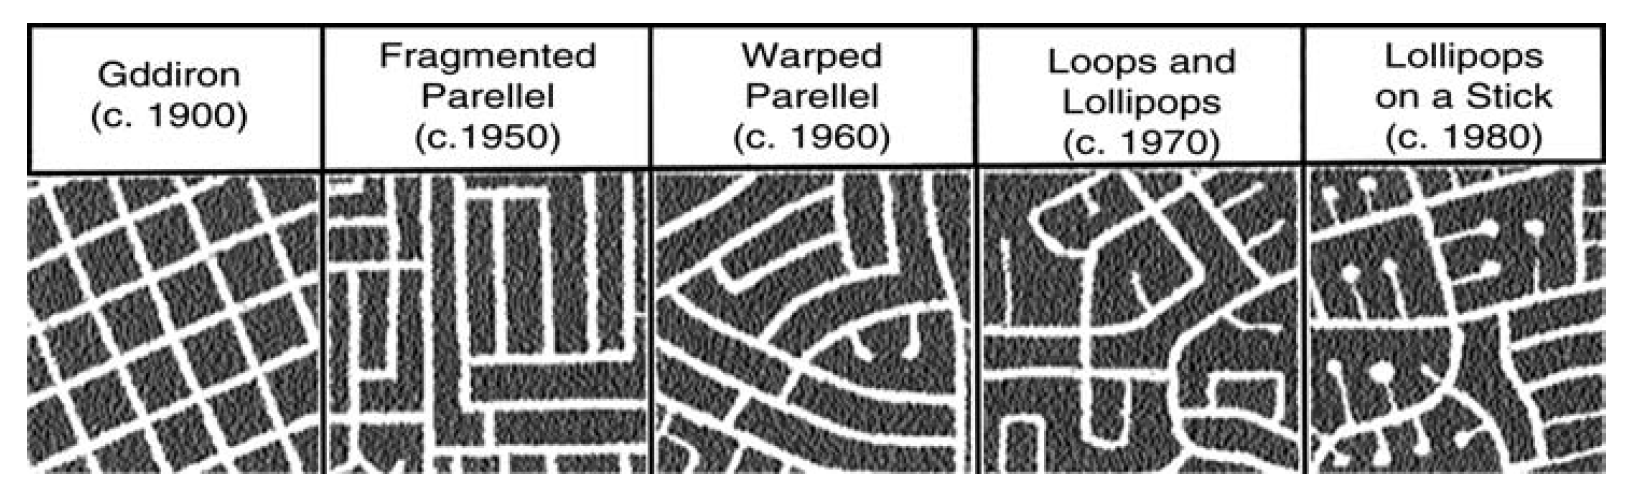
\includegraphics[width=0.95\textwidth,center]{picture/figure2.png}
\caption[Types of Street Patterns]{Types of street patterns. Source: \cite{Southworth:2003}}
\label{fig:streetpatterns}
\end{figure}

One major influencing factor to road network patterns is the typology (form or pattern) of the city themselves. To identify different road network types, [\cite{Snellen:2002}] study on the urban form, road network type, and mode choice for frequently conducted activities in the Netherlands is very useful. They distinguished between six principle urban forms, the concentric city, the lobe city, the linear polynuclear city, the concentric polynuclear city, the linear city, and the grid city as defined by [\cite{deKlerk:1980} \& \cite{Rottier:1980}]. On the basis of these six principles, they identified five elementary networks. Their classification is shown in Figure 2.33. Since this approach forms the one of the basis for the classification scheme adopted in this study, a brief description of each will be presented.

The radial network is suitable for all transportation modes. For example, in the Netherlands, it is the classic network for urban public transport, where buses radiate to and from the city center or railway station. When used as a network for the other transport modes, it offers direct accessibility to the city center. However, this network type is also prone to congestion problems. In theory, it can be applied to all morphological urban forms. [\cite{Snellen:2002}]

\begin{figure}[h]
\centering

\includegraphics[width=0.95\textwidth,center]{picture/figure3.png}
\caption[Elementary Transportation Networks]{Elementary transportation networks: (a) the linear network, (b) the radial network, (c) the ring, (d) the grid, and (e) the shifted grid. Source: \cite{Snellen:2002}}
\label{fig:transportnetworks}
\end{figure}

The ring network is frequently used mainly as a network for motorized transport. It offers the opportunity to concentrate a large amount of traffic on a single road, while other areas are relieved of traffic nuisance. In particular, city centers are often enclosed by a ring structure. This network type is not common for public transport in medium-sized cities, although it would provide good connections between city districts while avoiding a trip to and from the city center. For motorized and non motorized transport this network type can be applied to all morphological urban forms. For public transport, this network type is especially suitable for concentric polynuclear cities. [\cite{Snellen:2002}]

The (shifted) grid network is simple and direct, offers many choices of routes, and disperses traffic over many streets. Disadvantages of this network type are the many road crossings in the system. It is used mainly for motorized and non motorized transport. In theory, this network type is flexible and can be applied to all morphological urban forms. [\cite{Snellen:2002}]

[\cite{Chan:2011,Lima:2015}] divided a specific road network into four basic street network styles in their research, depicted in figure [\ref{fig:transportnetworks}].  The patterns observed in their results are often observed in cities and conform to the real-world design requirements of a street network. Their approach serves as one of the foundations for the classification scheme used in this study, and each will be briefly described below.

\begin{figure}[!ht]
\centering
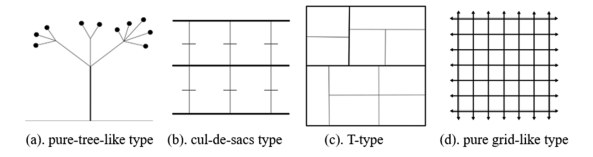
\includegraphics[width=0.75\textwidth,center]{picture/Cul de.png}
\caption[Abstract Structures of Four Kinds of Urban Street Networks]{Abstract structures of four kinds of urban street networks. Source: \cite{Han:2020}}
\label{fig:transportnetworks}
\end{figure}

Pure tree-like network pattern (Figure \ref{fig:transportnetworks}a). There are apparent backbone roads throughout the region and T-type cross and end-roads, forming a low-connected level network structure. This type of street network helps to protect residents' privacy and traffic stability, but it may be less robust than others.

The cul-de-sacs network pattern (Figure \ref{fig:transportnetworks}b). There are several trunks that run through a region with numerous end-roads. This type of network has good accessibility, but may be weaker in terms of interior connectivity than others.

T-type network pattern (Figure \ref{fig:transportnetworks}c). While this street network is similar to a pure grid-shaped network, the T-type intersections may improve trunk transportation efficiency while potentially reducing connectivity.

Pure grid-like network pattern (Figure \ref{fig:transportnetworks}d). Although this network is more connected than the others, transportation efficiency is typically lower due to the high number of intersections and short distances between them.

\section{Graph Networks}
A network is, in its simplest form, a collection of points joined together in pairs by lines. \cite{Newman:2010} "Network data structures for geographic information science (GIS) are methods for storing network data sets in a computer in order to support a range of network analysis procedures"[\cite{Curtin:2008}]. A network can represent a transportation or communications system, a utility service mechanism, or a computer system, to name only a few network applications" [\cite{Curtin:2008}]. Types of networks include flow networks and pure networks. Fischer explains flow networks will contain information on the flow of something within a network and a pure network represents any network's overall structure where the main concern are the topological relationships [\cite{Ficsher:2003}]. Additional examples of networks include computer networks, social networks, transport networks etc. Critical is the idea that a network by definition can be used to model and analyze linear features and their relationships. 

Networks, network models and network analysis are built upon the foundation of mathematics, typology and graph theory [\cite{Sovik:2014}]. Important contributions from graph theory are discussed in the next section and provide the foundation for characterizing networks, network analysis, and network pattern analysis.

A graph is an abstract representation of a set of elements and the connections between them [\cite{IntroductiontoGraphTheoryTrudeau:1994},\cite{Boeing:2017}]. A graph is made up of the following G = (N,E). In this example, G is the graph and the element N is interchangeably called the nodes (points) or vertices, and the connections between them E are called the edges (lines) or links. For consistency, this study uses the terms nodes and edges. The number of nodes within the graph (called the degree of the graph) is usually represented as n with the number of edges as m. Two nodes are adjacent if an edge connects them, two edges are adjacent if they share the same node, and a node and an edge is incident, if the edge connects the node to another node. A model like this is often depicted in the form of a picture. Figure \ref{fig:directedgraph}, provides an example of a simple graph where there are three vertices and three edges. As a principle, vertices do not loop back upon themselves[\cite{Duo:2002}]. 

\begin{figure}[h]
\centering
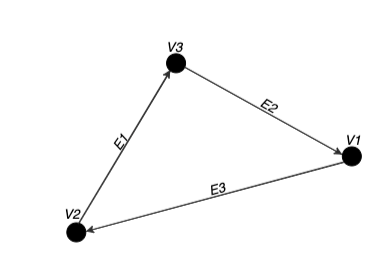
\includegraphics[width=0.95\textwidth,center]{picture/figure5.png}
\caption[Directed Graph]{Directed Graph}
\label{fig:directedgraph}
\end{figure}

An undirected graph's edges point mutually in both directions, but a directed graph, or digraph, has directed edges (i.e., edge E2 points from node V3 to node V1, but there is not necessarily a reciprocal edge V3,V1). A self-loop is an edge that connects a single node to itself. Graphs can also have parallel (i.e., multiple) edges between the same two nodes. Such graphs are called multigraphs, or multi digraphs if they are directed. An undirected graph is connected if each of its nodes can be reached from any other node. A digraph is weakly connected if the undirected representation of the graph is connected, and strongly connected if each of its nodes can be reached from any other node. A path is an ordered sequence of edges that connects some ordered sequence of nodes. Two paths are internally node-disjoint if they have no nodes in common, besides end points. A weighted graph's edges have a weight attribute to quantify some value, such as importance or impedance, between connected nodes. The distance between two nodes is the number of edges in the path between them, while the weighted distance is the sum of the weight attributes of the edges in the path. [\cite{Boeing:2017}]

Leonhard Euler published the first noted example of problem solving using graph theory in 1736. He used a graph in his seminal paper to solve the Königsber Bridge Problem. He sought a solution in his writings to the use of seven bridges linking two islands to the banks and each other. The problem was crossing each bridge once without doubling back. Interestingly, using graph theory, he showed that no solution to the problem existed[\cite{Duo:2002}]. 

Graph theory and its implementations have developed since the time of Euler. Today, network modeling tends to be based on the same underlying concepts used by Euler, but the amount of knowledge that can be modeled and the complexity of the networks have expanded with the introduction of computers and GIS. Familiar examples include social networks (where individuals are the nodes and their interpersonal connections are the edges) and the World Wide Web (where web pages are the nodes and hyperlinks leading from one to another are the edges). A complex network (the configuration and arrangement of its nodes and edges) is one with a non-trivial topology, i.e. the topology is neither entirely regular nor totally random. The majority of big real-world networks [\cite{Newman:2010}] are dynamic. Complex spatial networks, i.e. complex networks with nodes and/or edges embedded in space, are of special importance in this analysis [\cite{OSullivan:2014}]. A street network, as well as railways, power grids, and water and sanitation networks, is an example of a dynamic spatial network of both nodes and edges embedded in space[\cite{Barthelemy:2011}]. [\cite{Newman:2003}] paper, "The Structure and Role of Complex Networks," is recommended for more in-depth review[6].

\section{Road network as Graphs}
Road networks are usually modeled as graphs, with nodes representing intersections and dead ends, and edges representing street segments connecting them [\cite{Barthelemy:2008, Cardillo:2006, Lin:2013, Marshall:2018, Porta:2006}]. These edges are embedded in space and have a bearing of both length and compass [\cite{Barthelemy:2011}]. The current research models urban street networks with potential  self-loops as undirected nonplanar multigraphs. Though most-faithfully guided graphs reflect flow restrictions (such as vehicular traffic on one-way roads), undirected graphs best model urban structure by referring to street segments (i.e. the linear sides of city blocks) by 1:1. Although many street networks are roughly planar (with very few overpasses or underpasses), by accommodating certain bridges and tunnels which also occur, nonplanar graphs offer more detailed models [\cite{Boeing:2018, Eppstein:2008}].

Data used to study these networks typically comes from the shapefiles of digitized streets. The data can be generated by individual local, state or federal entities within each country, but the criteria for digitization and availability of the data differ. As a result, cross-sectional street network orientation and entropy analysis tended to be confined to unique geographic areas or to analyze small samples (Boeing, 2019). Today, however, OpenStreetMap offers a new alternate data source. OpenStreetMap is a global collaborative mapping initiative comprising highways, houses, services, and other spatial features. Although the quality of its data varies somewhat across countries, its street data is generally of high quality,  especially in cities [\cite{Barrington-Leigh:2017, Barron:2014, Zielstra:2013}]. The OpenStreetMap data source gives the ability to conduct cross-sectional research into the form and layout of street networks around the world. Researchers have recently studied the order and disorder of the street network through the  circuity and orientation entropy. Circuity focuses on the measures of the street curvature and how it applies to other urban network patterns [\cite{Boeing:2019, Giacomin:2015, Levinson:2009}]. The orientation entropy quantifies and visualizes the entropy of street orientations in order to determine how ordered they are [\cite{Courtat:2011, Gudmundsson:2013, Mohajeri:2013, Mohajeri:2013:1, Mohajeri:2014, Mohajeri:2012}]. In their research, [\cite{Louf:2014}] studied the geometry of city blocks around the world as a function of block size and form factor, clustering them together to define the differences between US and European cities. However, little is understood about cross-sectional patterns in the spatial orientation and ordering of road networks around the world. This thesis draws on this previous analysis into circuitry, order, and entropy by building on OpenStreetMap data to analyze cities around the world and investigate similarities in their patterns and relationships.

A spatial network is planar if it can be represented with its edges intersecting only at nodes in two dimensions. For example, a road network may be planar (especially in some small scales), but most road networks are non-planar due to grade-separated expressways, overpasses, bridges, and tunnels [\cite{Boeing:2017}]. In spite of this, a large number of existing quantitative analyses of urban street networks represent them as planar graphs for tractability [\cite{Barthelemy:2008, Buhl:2006,Cardillo:2006, Masucci:2009, Strano:2013}], since bridges and tunnels are comparatively rare (in some places), so the networks are roughly planar. However, this oversimplification of tractability planarity can be needless and may cause methodological problems. The street networks mentioned so far are known as primal graphs that represent nodes as intersections and edges as street segments. This thesis, however, focuses on primal graphs because they preserve all the geographical, spatial, and metric information essential to the urban form and design that dual representations discard for a  street network as all the such as the length, shape, circuity, width, etc. The primal graph, on the other hand, represents all the spatial characteristics of a street network. Using Primal graphs may be a better approach to analyzing spatial networks where geography matters, since the physical space underlying the networks themselves contains the relevant information that cannot exist in the topology of the network alone [\cite{Ratti:2004}].

\subsection{Evaluation Metrics of Road Networks}
Road network topology is defined as the spatial arrangement of roads at a given location [\cite{Rodrigue:2016}]. It is conventionally evaluated by the measures of gridness, treeness, ringness, webness, [\cite{Barthelemy:2011, Buhl:2006, Gudmundsson:2013, Xie:2007}] and typology [\cite{Louf:2014}]. Recent advances in topology, graph theories and the growth in computing ability has paved the way for more advanced methods for quantitative analysis of road network patterns [\cite{Jiang:2004, Cardillo:2006, Bavelas:1948}].

In their research, [\cite{Xie:2007, Levinson:2012}], pointed out that the two fundamental structures commonly observed in the planar transport network include the tree-like network and grid-like network. In this regard, [\cite{Noda:1996}] introduced the grid-tree-proportion index (GTP index) as a new mathematical measure uniting the alpha and gamma indices used to jointly evaluate the grid pattern, tree pattern, and other road network patterns that do not belong to either of the two categories  highlighted [\cite{Usui:2011}]. The approach is also used to quantify the formation, coherence and connectivity of road network patterns [\cite{Gogoi:2013, Usui:2011, Wang:2017}]. In addition, it is used to assess the efficiency of traffic flow or movement in the road network. The GTP index ranges from the lowest value of 0 to the highest value of 1. The GTP index coefficient is computed by substituting the following formula.

\begin{equation}
{GTP}=\frac{e-V+1}{\left(\sqrt{V-1)^{2}}\right.}
\end{equation}

Where:
GTP $=$ Grid Tree Pattern
$\mathrm{e}=$ Total number of edges (Links)
$\mathrm{V}=$ Total number of vertex (Nodes)
{Source: \cite{Tini:2018}}

Road networks considered to be primal, non-planar, weighted multi-digraphs with self-loops can be characterized, described and evaluated by both metric and topological measures. Extended concepts and algorithms can be found in [\cite{Newman:2010, Barthelemy:2011}]. 

Measured in terms of length and area, the metric structure represents common transportation variables [\cite{Cervero:1997, Ewing:2010}]. [\cite{Boeing:2017}], defined the following major metric measures for density as “average street length, mean edge length (in spatial units such as meters) in the undirected representation of the graph which all act as the linear proxy for block size and shows how fine-grained or coarse-grained the network is. Node density is the number of nodes divided by the area covered by the network. Intersection density is the node density of the group of nodes with more than one street emanating from them (excluding dead-ends). The edge density is the sum of all edge lengths divided by the area, and the physical street density is the sum of all edges in the undirected representation of the graph divided by the area”. All these density measures give a further indication of how fine-grained the network is. Finally, the average circuity divides the sum of all edge lengths by the sum of the great-circle distances between the nodes incident to each edge [\cite{Giacomin:2015}]. This is the average ratio between the length of the edge and the straight-line distance between the two nodes it connects.

Topological measures of the structure of a street network often indicate the configuration, connectedness, and robustness of the network as well as how these characteristics are distributed. The average node degree, or mean number of edges that are incident to each node, quantifies the connectivity of each node on average. “Similarly, but more precisely, the average streets per node measures the mean number of physical streets emanating from each intersection and dead-end. This adapts the average node degree to the physical form rather than to the directed circulation” [\cite{Boeing:2017}]. The statistical and spatial distributions of the number of streets per intersection describe the type, prevalence, and dispersion of the connectivity of all intersections in the network. Connectivity measures the minimum number of nodes or edges to be removed from a connected graph in order to disconnect it. It is considered to be a measure of resilience, since complex networks with high connectivity offer more routing options for agents and are more robust to failure. However, node and edge connectivity is less effective for approximately planar networks like street networks: most street networks will have the connectivity of 1, because the presence of a single dead-end means the removal of just one node or edge can disconnect the network. More usefully, the average node connectivity of a network the mean number of internally node-disjoint paths between each pair of nodes within the graph represents the expected number of nodes that has to be removed to disconnect a randomly selected pair of non-adjacent nodes [\cite{Beineke:2002}]. As [\cite{OSullivan:2014}] explains, both spatial integration and approximate planarity greatly limits a network’s distance, degrees and connectivity. Other measures of connectedness within a network such as intersection density, node degree distribution, and centrality/clustering (discussed in the next paragraph) can better capture the nature of a street network's connectedness than node or edge connectivity. Low connectedness networks can have several single points of failure, making the system especially vulnerable to perturbation. This is evident in urban design by the way of permeability and choke points, for instance, traffic jams can occur and circulation networks can fail if circulation within the network is forced through single points of failure. [\cite{Hajrasouliha:2015}] linked connectedness to pedestrian volume within a street network.

In addition to being able to better capture the nature of the connectedness of a road network than node or edge connectivity, clustering measures also show the topological structure and distribution of a street network. Boeing 2017, describes a node’s clustering coefficient as “the ratio of the number of edges between its neighbors to the maximum possible number of edges that would exist between these neighbors”. The weighted clustering coefficient is used to calculate the connectivity and complexity from how thoroughly the neighborhood of a given node is connected together, since it weighs the connectivity and complexity ratio from edge length and the average clustering coefficient as the mean of the clustering coefficients of all the nodes in the network. The weighted clustering coefficient was extended to neighborhoods within an arbitrary distance by [\cite{Jiang:2004}] to make it more applicable to urban street networks. The importance of nodes in a network is indicated by the Centrality. [\cite{Barthelemy:2004}], describes the Betweenness centrality as the evaluation of the number of shortest paths that pass through each node or edge. The maximum betweenness centrality in a network specifies the  proportion of shortest paths that pass through the most important node/edge. This is a measure of resilience: networks with a high maximum betweenness centrality are more vulnerable to failure if the single choke point fails. The average betweenness centrality is the mean of all the betweenness centralities in the network [\cite{Barthelemy:2011}]. In their work, [\cite{Barthelemy:2013}] used the betweenness centrality to identify top-down interventions against the bottom-up self-organization and evolution of Paris's urban network pattern. Closeness centrality represents, for each node, a reciprocal sum of the distance from that node to all other nodes in the network: that is, nodes rank as more central if they are on average similar to all other nodes. Finally, PageRank, developed by [\cite{Brin:1998}] is the algorithm used by Google to rank web pages. The PageRank algorithm is known to be a variant of the network centrality, namely the eigenvector centrality. PageRank can also be extended to street networks, as it ranks nodes on the basis of the structure of incoming links and the rank of the source node. [\cite{Agryzkov:2012, Chin:2015}]

\section{Graph Similarity Measures}
As a result of the recent developments on graph matching, different algorithms have been proposed to solve the problem of comparing graph-based representation [\cite{Bunke:2000}] . Though little has been explored in this regard for road network representations, these graph matching algorithms can be adapted in order to support the calculation of similarities. Some of the most important measures are presented in the following paragraphs. It is also important to emphasize that there is not a single criterion to choose the best measure since their performance does greatly depend on the characteristics of the graph [\cite{Papadimitriou:2010}]. As such, experimentation is the most appropriate way to select the best algorithm for the problem at hand [\cite{Jouili:2010}]. 

These following descriptions below aren't comprehensive descriptions of every graph comparison method in use today, but they do show some similarities between them.

\subsection{Graph Edit Distance / Graph Isomorphism}
Graph isomorphism is one method for evaluating graph similarity. If two graphs are isomorphic, they are similar [\cite{Pelillo:1999}], or one is isomorphic to a subgraph of the other , or they contain isomorphic subgraphs. The disadvantage of graph isomorphism is that the exact versions of the algorithms are exponential making them inapplicable to today's large graphs.  The graph edit distance is a variant of the graph isomorphism problem, in which the goal is to transform one graph into another by performing a series of operations (additions, deletions, substitutions of nodes or edges, and reversions of edges). This method assigns a cost to each operation and seeks to find the operation sequence that will minimize the cost of matching the two graphs.[\cite{Koutra:2011}]

GED (graph edit distance) is a more flexible similarity measure that contemplates the differences in edges and nodes as well as the set of associated weights [\cite{Gao:2010}]. There are many adaptations of GED; however, the use of the bipartite variation of GED to limit algorithm complexity has been used as much as possible [\cite{Manrique:2018}]. 

The most basic graph distances and extensions aggregate element-by-element comparisons between the adjacency matrices of two graphs; [\cite{Golub:2013, Jaccard:1901, Hamming:1950, Gao:2010, Wallis:2001}]; because these methods are known to explicitly depend on the node labeling scheme (and are therefore not invariant under graph isomorphism [\cite{Chowdhury:2017}], their utility when comparing graphs with unknown labels  may be limited (e.g. graphs sampled from random graph ensembles). Several measures collect empirical distributions [\cite{Carpi:2011}] or a “signature” vector [\cite{Berlingerio:2012}] from each graph and compute the distance between them (using the Jensen-Shannon divergence, Canberra distance, earth mover’s distance, and other measures [\cite{Emmert-Streib:2016}], which allows for the comparison of graphs with different sizes. [\cite{Bagrow:2019}].

\subsection{Signature Similarity}
Signature similarity [\cite{Papadimitriou:2010}] is another graph similarity metric to consider. Using the node weights, the method attempts to generate a signature vector of 1s and 0s for each graph. The vectors are then compared by counting the number of matches between them. It normalizes the result and provides similarity measurements between 0 and 1.

\subsection{Spectral Distance}
Another approach is comparing the spectral properties of certain matrices characterized by graphs [\cite{Jurman:2015}], such as the non-backtracking matrix [\cite{Torres:2019, Mellor:2019}] or Laplacian matrix [\cite{Jurman:2011}], which is known as spectral distance. The relevant spectral properties associated with these distances are invariant under graph isomorphism. [\cite{Chowdhury:2017, vanSteen:2010}]. Some of these graph distance measures have been proven to be metrics (that is, they satisfy properties like triangle inequality, etc.) [\cite{Deza:2009}], while others have not.

\subsection{Feature-based Distance}
Looking at specific "features" of the graph, such as the degree distribution, betweenness centrality distribution, diameter, number of triangles, number of k-cliques, and so on, is one method for comparing graphs. For vector-valued graph features (such as degree distribution), one could also consider the vector as an empirical distribution and use the sample moments as graph features (or quantiles, or statistical properties). A feature-based distance is one that compares graphs by comparing such features.

Of course, all of the methods discussed thus far are feature-based in general; however, in the special case where the features occur as values over the space V V of possible node pairings, they are often referred to as  matrix distances. Similarly, if the feature in question is the spectrum of a specific matrix realization of the graph, the method is referred to as a spectral distance.

[\cite{Berlingerio:2012}] proposes NETSIMILE, which is a feature-based distance with the  focus on local and egonet-based features (e.g., degree, volume of egonet as fraction of maximum possible volume, etc.). When k features are used, the method generates a feature-vertex matrix of size k n. The associated feature matrix generated is then reduced to a "signature vector" (a process referred to as "aggregation" by the authors of [\cite{Berlingerio:2012}] that consists of the mean, median, standard deviation, skewness, and kurtosis of each These signature vectors are then compared to determine the distance between graphs.

Feature-based methods for comparing graphs are popular in the neuroscience literature, in particular [\cite{Bassett:2008, Kaiser:2011}]. The authors [\cite{vandenHeuvel:2013}] compared the functional connectivity networks of patients with and without schizophrenia using graph features such as modularity, shortest path distance, clustering coefficient, and global efficiency. Using standard statistical techniques, the statistics for these features for the control and experiment groups are aggregated and compared.

\subsection{Maximum Common Subgraph}
A different approach to graph similarity is the Maximum Common Subgraph. Different variations that have been proposed for the MCS (Maximum common subgraph) algorithm [\cite{Bunke:1998}]. The MCS is the largest subgraph that is common in the considered graphs. Different metrics use the size of the MCS as an indicative of similarity. The size of a sub-graph can be measured in several ways, but the focus of this thesis will be on the number of nodes. This method is especially useful in biological and chemical analysis [\cite{Willett:1999}], as well as the graph kernel approach. Chapter 3 goes into greater detail about its application.

\subsection{Vertex Edge Overlap}
VEO (vertex edge overlap) [\cite{Papadimitriou:2010, Manrique:2018}] is a basic strategy that measures the similarity between two graphs by calculating the overlap between their edges and nodes, ignoring the edge or node weights.  This method  attempts to simplify the graph matching problem by counting the total number of vertices and edges that match and dividing the result by the sum of the total number of vertices and edges on each graph. This factor is multiplied by 2 in order to normalize the result appropriately. [\cite{Manrique:2018}]

\begin{equation}
V E O\left(G, G^{\prime}\right)=2 \frac{\left|V \cap V^{\prime}\right|+\left|E \cap E^{\prime}\right|}{|V|+\left|V^{\prime}\right|+|E|+\left|E^{\prime}\right|}
\end{equation}
Source: \cite{Manrique:2018}

Because it only uses variables from the graph, this algorithm can be applied to any graph structure. Even so, it is an extremely limited approach because it does not take into account information such as vertex or edge weight or path information. This method is based on a simplified version of the GED (Graph edit distance) algorithm and is normalized to a scale of 1 to 0, with 1 being completely similar and 0 being completely dissimilar. The complexity of this algorithm is O(V + E) because it only requires a single iteration over the sets of one of the graphs to find the matching pairs in both vertices and edges.


\subsection{Graph Clustering}
The term Graph clustering is currently used in literature for two distinct and unrelated interpretations, each of which may be of concern to researchers working in the field of Pattern Recognition: in the first sense, graphs are used to represent each of the items to be clustered, so clustering is done on a collection of graphs. In the second sense, which is the most commonly found, according to [\cite{Foggia:2014}] “a single graph is used to represent the structure of the space to which the objects belong with a node for every object and edges encoding the relationships between pairs of objects usually a similarity or a distance measure is related to each edge; in this case, the clustering is carried out by splitting the set of nodes of the graph according to some criterion”. Of particular interest to this study is the clustering of graphs which is used to find the similarity between different road network patterns represented as graphs.

\subsection{Clustering of Graphs}
For the clustering of graphs, [\cite{Gunter:2002}] proposed an application to graphs with the Unsupervised Learning Vector Quantization (LVQ) algorithm. The algorithm uses Graph Edit Distance to determine the distance between an input graph and a prototype cluster and an initial GED-based algorithm that determines the weighted combination of two graphs (by calculating the minimum number of editing operations to transform the first graph to the second, and then by choosing a subset of these operations depending on the weight), which is used for updating the winning prototype. The same authors suggested an extension of this approach in 2003 [\cite{Gunter:2003}], adding a series of validity indices for clustering to pick the optimum number of LVQ nodes. [\cite{Serratosa:2002}] proposed an algorithm based on Function-Described Graphs for the clustering of graphs, which are Attributed Relational Graphs, extended with information about the node and edge joint probability constraints. The algorithm is based on an incremental, hierarchical clustering strategy. [\cite{Brijnesh:2011}] in their paper presented a method for the clustering of graphs based on the Vector Quantization with the k-Means algorithm. To perform the quantization, the suggested algorithm uses the integration of graphs into Riemannian orbit folds, based on Graph Edit Distance. The authors explored in-depth the theoretical characteristics of the proposed solution, pointing out some necessary conditions for the optimality of the clustering found and for statistical consistency; the authors also discussed the effect of potential approximations on reducing the cost of computing.

\begin{figure}[!ht]
\centering
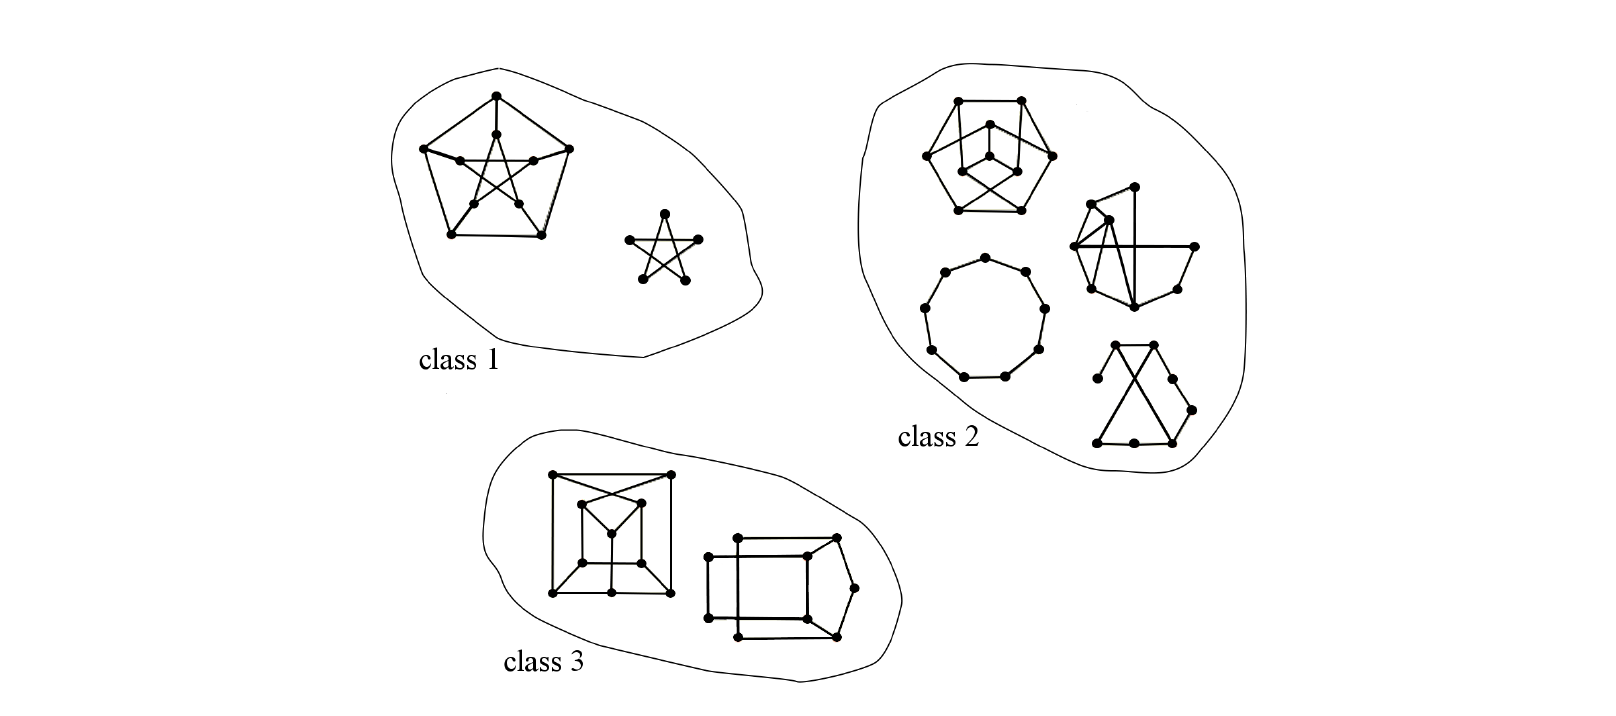
\includegraphics[width=0.95\textwidth,center]{picture/figure6.png}
\caption[Clustering of Graphs]{Clustering of graphs: each of the objects to be clustered is represented by a graph. Source: \cite{Foggia:2014}}
\label{fig:clusteringgraphs}
\end{figure}

\subsection{Graph Kernels}
A graph kernel is a function that maps a few graphs to a real number, and has similar properties to the vector-defined dot product. More formally, if we denote the space of all the graphs with G, a graph kernel is a function k such as:

\begin{equation}
k: \mathbb{G} \times \mathbb{G} \longrightarrow \mathbb{R}
\end{equation}
\begin{equation}
k\left(G_{1}, G_{2}\right)=k\left(G_{2}, G_{1}\right) \quad \forall G_{1}, G_{2} \in \mathbb{G}
\end{equation}
\begin{equation}
\sum_{i=1}^{n} \sum_{j=1}^{n} c_{i} \cdot c_{j} \cdot k\left(G_{i}, G_{j}\right) \geq 0
\end{equation}
\begin{equation}
\forall G_{1}, \ldots, G_{2} \in \mathbb{G}, \forall c_{1}, \ldots, c_{n} \in \mathbb{R}
\end{equation}

In the equation 2.5.3 above, the function k is required to be symmetric, while Equation's 2.5.4 and 2.5.5 respectively requires it to be positive semi-definite. Source: \cite{Foggia:2014}

A graph kernel can be viewed informally as a measure of the similarities between two graphs; however, its formal properties allow a kernel to replace a vector dot product with many vector-based algorithms (and other dot-related functions, such as the Euclidean standard) that use this operator. Thanks to the Mercer theorem, kernels have long been used to extend linear algorithms operating on vector spaces to nonlinear cases: given the kernel function defined on compact Hausdor space X, vector space V and mapping between X and V are used in such a way that the kernel value calculated on two points in X is equal to the dot product of the corresponding points in V. While the theorem of Mercer does not apply to graph kernels, the latter can be used in practice as a theoretically sound way to extend a vector algorithm to graphs. The efficiency of these algorithms, greatly depends on the appropriateness of the notion of similarity expressed within the graph kernel (with relevancy to the task at hand). [\cite{Foggia:2014}] 

[\cite{Kashima:2003}], in their paper, they proposed the idea of marginalized kernels, a probabilistic approach for defining a kernel based on the introduction of specialized hidden variables for the graph domain. In this case, the hidden variable is a sequence of node indices generated on one of the graphs according to a random walk. Provided the value of the concealed variable, the sequence kernel is calculated using the sequence of nodes and edges visited; the marginalized kernel is calculated by estimating the estimated value of the sequence kernel (concerning the combined distribution of the hidden and visible variables). [\cite{Mahe:2009}] extended this technique to trees and presented a molecular data application. To avoid the exponential cost of enumerating all the paths in a graph, the authors proposed a scheme to use only the shortest path between any pair of nodes since the shortest paths can be calculated in polynomial time. [\cite{Karsten:2005}] presented a graph kernel based on paths instead of walks (a path is a walk without repeated nodes). [\cite{Neuhaus:2006}], introduced three graph kernels based on Graph Edit Distance in their paper. The first kernel requires a zero pattern to be chosen, a graph that will act similarly to a null vector with respect to the kernel. The authors found that the kernel fulfills the theoretical requirements of a kernel function, but it's functional performance is significantly influenced by the choice of the zero patterns. The authors then introduced two other kernels, obtained over a set of zero patterns from the sum and the product of the first kernel, and proved that they have the same theoretical properties but are more stable in choosing these patterns.

[\cite{Neuhaus:2009}] in their paper,  presented three possible ways to use Graph Edit Distance in the definition of a kernel. The first way is a diffusion kernel, which transforms the edit distance matrix into a positive definite matrix that satisfies the properties of the kernel, but has the inconvenience that the set of graphs on which it is applied must be finite and known a priori. The second way is a convolution kernel which is based on the decomposition of the edit path between the two graphs into a sequence of substitution operations; this method provides a definition for a kernel between two graphs, given the kernel for individual substitutions. The only downside is the exponential complexity of the number of nodes for which an estimate is proposed by the authors. A random walk kernel is the third way, where the Graph Edit Distance is used to denote a fuzzy graph of the product from which a kernel is obtained that evaluates the local similarity of the corresponding parts of the two graphs.

[\cite{Gauzere:2012:1}] paper introduces two graph kernels. The first is based on the Graph Edit Distance, called the Laplacian Kernel. The operation of the product extracted from the Graph Edit Distance is not guaranteed to be positive definite, and thus does not have the formal properties of the kernel; thus, the authors recommended a technique to obtain a positive definite matrix from the distance matrix, which is then used as the kernel. The second kernel, known as the treelet kernel, is based on treelets, which are all potential trees with less than a fixed number of nodes (up to 6 nodes are considered in the papers); the kernel is determined by counting the occurrences of each treelet in the graphs. Only unattributed graphs can use this kernel, while the Laplacian kernel can also be used for graphs with node and edge attributes. The same authors also later suggested a kernel that is also based on treelets but uses a treelet edit distance instead of merely counting their occurrences to equate the treelets in one graph with those in the other, so as to be tolerant of minor deformations of the graphs. In their article, [\cite{Grenier:2013}]suggested a different treelet-based kernel, especially developed for applications in chemoinformatics, which often integrates knowledge within the graph on the position of each treelet. [\cite{BarbaraStrug:2011}]proposes a kernel based on combining a tree kernel with a classical graph kernel, explicitly developed for hierarchical graphs.

\chapter{Methodology and Implementation}
    %%%%%%%%%%%%%%%%%
% Methodology and Implementation %
%%%%%%%%%%%%%%%%%

This study builds on a rich body of road and graph network research by analyzing the similarities between different road networks.

\begin{figure}[h]
\centering
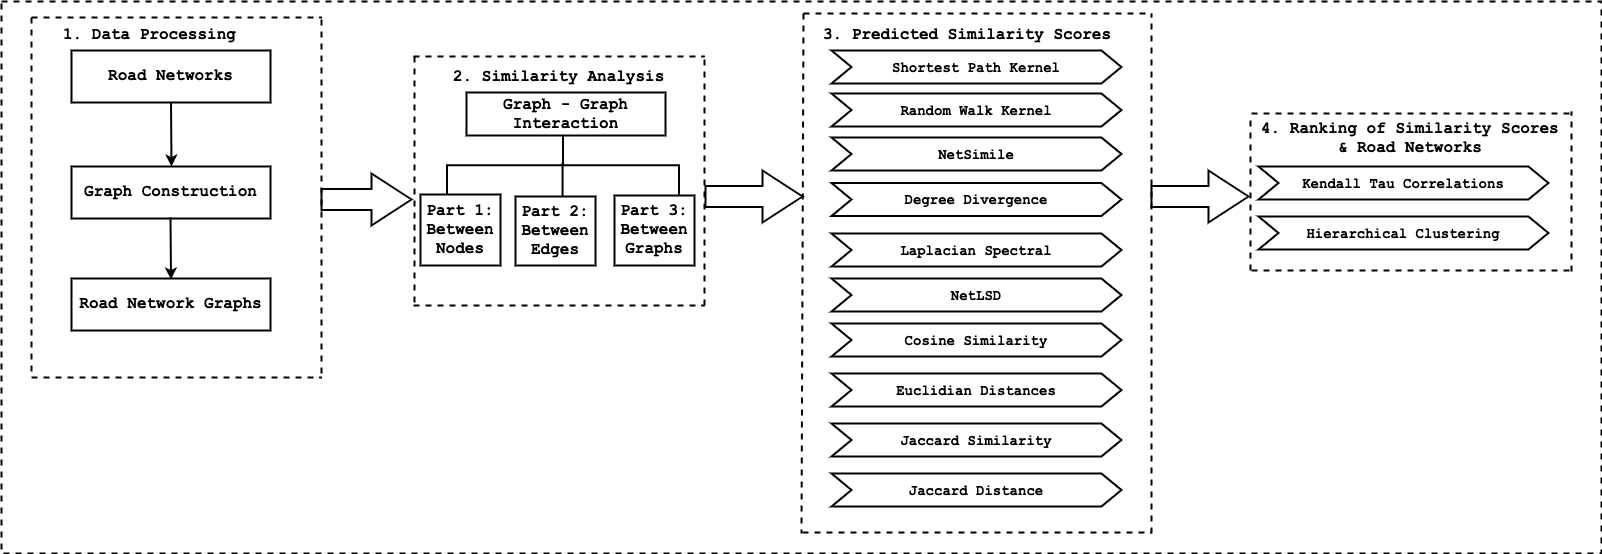
\includegraphics[width=1.25\textwidth,center]{picture/flows.png}
\caption[Methodology Workflow]{Methodology Workflow}
\label{fig:Methodology Workflow}
\end{figure}


\section{Data}
\begin{figure}[h!]
\centering
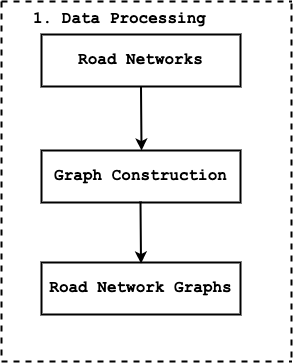
\includegraphics[width=0.35\textwidth,center]{picture/flow1.png}
\caption[Data Processing Workflow]{Data Processing Workflow}
\label{fig:Data Processing Workflow}
\end{figure}

The similarity analysis will be performed on 22 major cities worldwide, following [\cite{Louf:2014}] sampling strategy of selecting cities based on a balance of high population, regional significance, and some stratification to ensure geographical diversity within regions. The 22 sampled cities span across Africa, Asia, Australia, Europe, Middle East, North America and South America. As a result, all samples represent a diverse range of historical, cultural, developmental, and design paradigms. Of course, there is no universally accepted definition of "city" or its spatial jurisdiction throughout the world, as these differ between countries for historical and political reasons. The aim is for consistency, by trying to use each study site’s closest approximation of a “municipality” for the city limits. Once these study sites are defined, the OSMnx software is used to download the data and road network type for each city from OpenStreetMap. Due to its high-quality worldwide coverage, OpenStreetMap (OSM) is a collaborative online mapping platform commonly used by researchers. OpensStreetMap also provides extensive, user-contributed, open data on transport networks. OpenStreetMap’s raw data contain many interstitial nodes in the middle of street segments (forming an expansion graph) to allow streets to curve through space via a series of straight-line approximations. OSMnx automatically simplifies the topology for each graph to retain nodes only at intersections and dead-ends, while retaining for each edge their true spatial geometry. This provides accurate intersection counts and edge length measures for comparison between  networks with planar and nonplanar representations.

\section{Selected Cities}
As previously stated, this study selected 22 urban road networks from around the world, which are listed in Table \ref{tab:Selected Cities}, along with their characteristic urban form and Node and Edge size count, to determine whether road network types in different regions share any similarities. As discussed in Chapter 2, road network data sets can be classified into five basic pattern types: tree-like, grid, cul-de-sac, linear, and radial. Despite the fact that the number of 22 data sets appears to be small, this study believes that these data sets demonstrate the dependability of the study objectives and results for the following reasons. First, despite the fact that the appearance of the city varies greatly, the main pattern differences in the urban road network can be found in the shape of intersections and the density of the road network. The only thing that needs to be determined in a classification study are the characteristics of the reference network; it is not necessary to identify all of the networks one by one. Over Reliance on large-scale statistical data may make accurate identification of road network features impossible, as some features may become submerged in the massive statistical values [\cite{Han:2020}]. Furthermore, approximately 40 road network samples were chosen for this study on a preliminary basis. To clearly express the road network boundary and data distribution, city samples with similar patterns and parameters were removed.
Furthermore, each sample area was limited to two square kilometers for ease of comparison. (one kilometer by one kilometer)


% Please add the following required packages to your document preamble:
% \usepackage{graphicx}
% \usepackage{lscape}
\begin{landscape}
\begin{table}[]
\resizebox{\textwidth}{!}{%
\begin{tabular}{|l|l|l|l|l|l|}
\hline
\multicolumn{1}{|c|}{\textbf{City}} &
  \multicolumn{1}{c|}{\textbf{Country}} &
  \multicolumn{1}{c|}{\textbf{Road Network Pattern (Drive)}} &
  \multicolumn{1}{c|}{\textbf{Continent}} &
  \multicolumn{1}{c|}{\textbf{Nodes}} &
  \multicolumn{1}{c|}{\textbf{Edges}} \\ \hline
Jerusalem                       & Israel      & Cul-de-sac   & Asia          & 387  & 671  \\ \hline
Amsterdam                       & Netherlands & Cul-de-Sac   & Europe        & 547  & 1049 \\ \hline
Nairobi                         & Kenya       & Radial       & Africa        & 410  & 793  \\ \hline
District of Columbia            & USA         & Grid         & North America & 461  & 1167 \\ \hline
Berlin                          & Germany     & Grid         & Europe        & 270  & 665  \\ \hline
Helsinki                        & Finland     & Grid         & Europe        & 417  & 913  \\ \hline
Toronto                         & Canada      & Grid         & North America & 325  & 827  \\ \hline
St, Petersburg, Florida         & USA         & Grid         & North America & 353  & 1069 \\ \hline
Belgrano, Buenos Aires          & Argentina   & Grid         & South America & 369  & 697  \\ \hline
Roda Island, Cairo              & Egypt       & Radial       & Africa        & 1036 & 2520 \\ \hline
Jumeirah Islands, Dubai         & UAE         & Linear       & Asia          & 93   & 198  \\ \hline
Jakarta                         & Indonesia   & Linear       & Asia          & 242  & 403  \\ \hline
Sydney                          & Australia   & Linear       & Australia     & 66   & 121  \\ \hline
Connaught Place, New Delhi      & India       & Radial       & Asia          & 391  & 853  \\ \hline
Champs-Elysees, Paris           & France      & Radial       & Europe        & 443  & 886  \\ \hline
Athens                          & Greece      & Shifted Grid & Europe        & 780  & 1405 \\ \hline
Palmanova,Friuli-Venezia Giulia & Italy       & Radial       & Europe        & 172  & 405  \\ \hline
Surulere, Lagos                 & Nigeria     & Radial       & Africa        & 280  & 629  \\ \hline
Ejecutivo, Mexico City          & Mexico      & Shifted Grid & South America & 530  & 1260 \\ \hline
Copenhagen                      & Denmark     & Shifted Grid & Europe        & 421  & 875  \\ \hline
Mumbai                          & India       & Tree         & Asia          & 363  & 826  \\ \hline
City of Westminster, London     & UK          & Tree         & Europe        & 607  & 1346 \\ \hline
\end{tabular}%
}
\caption{Selected Cities}
\label{tab:Selected Cities}
\end{table}
\end{landscape}

\begin{figure}[h!]
\centering
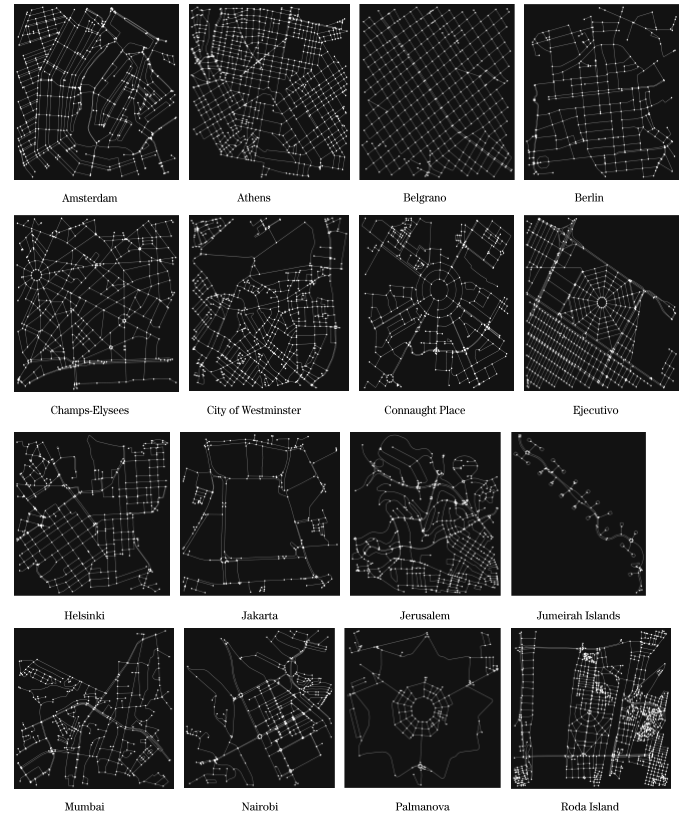
\includegraphics[width=1.0\textwidth,center]{picture/Graphs1.png}
\end{figure}

\begin{figure}[h!]
\centering
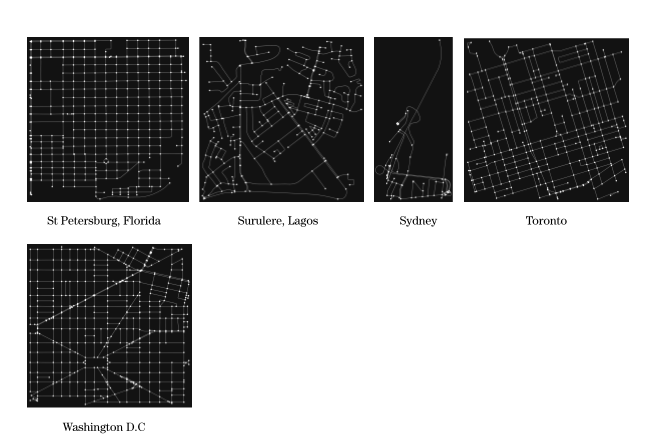
\includegraphics[width=1.0\textwidth,center]{picture/Graphs2.png}
\caption[Road Network Graphs]{Road Network Graphs}
\label{fig:roadnetworkgraphs}
\end{figure}

\section{Road Network Similarity Metrics}
All the network-similarity metrics used for this study are categorized based on two criteria. First, at what level of the network does the method operate? Second, what type of comparison does it use? 

For the first criteria, 3 levels are defined, they are micro, mezzo, and macro. As their names imply, at the micro-level, a metric extracts features at the node level;1 at the mezzo-level, the metric extracts features from communities; and at the macro-level, it extracts features from the global/network level[\cite{Soundarajan:2014}].


For the second criteria, there are 3 types: vector-based, classifier-based, and matching-based. For this study, we will be using the vector-based and classifier-based types, which are described below. 

For the Vector-based metrics, feature vectors F1 and F2 are assigned to each network G1 and G2, respectively. They define the similarity between G1 and G2 as $1-Canberra(F1, F2)$ [\cite{Richards:2010}].

For the Classifier-based metric,  a fixed number of structures is first identified within each network (such as random walks, communities, or node neighborhoods). FA feature vector describing the structural properties of each of these structures (e.g., the number of edges within a node neighborhood) is calculated for each of these structures, and the feature vectors are then labeled with the name of their respective network [\cite{Soundarajan:2014}]. Cross-validation is then used afterward to determine if a Support vector machine (SVM) can accurately distinguish between the feature vectors from network G1 and the feature vectors from network G2. The test set in each round of cross-validation contains feature vectors from G1 and G2; resulting in a length-2 feature vector (respectively, F1 and F2) describing the fraction of feature vectors from that network that were classified as belonging to G1 and the fraction that were classified as belonging to G2. The similarity between G1 and G2 is defined as $1-Canberra(F1, F2)$. The SVM will be unable to distinguish between the two classes of feature vectors if G1 and G2 have very similar local structures, and F1 and F2 will be very similar. The distance between F1 and F2 will be very short, resulting in a high degree of similarity. If G1 and G2 have drastically different structures, the SVM will have a high classification accuracy but a low similarity score.

For the matching-based metric, see [\cite{Soundarajan:2014}] which goes into detail how this approach is described and can be applied. 

Table \ref{tab:Road Network Similarity Methods} categorizes all road network-similarity metrics based on the two criteria mentioned above. Each of these 10 metrics is briefly described below. Based on previous studies and research [\cite{Soundarajan:2014}], because macro-level metrics consider the entire network at once, rather than local sub-structures, it is not possible for such metrics to be classifier- or matching-based.

\begin{table}[!h]
\centering
\begin{tabular}{|p{3cm}|p{3cm}|p{3cm}|p{3cm}|}
\hline
& \textbf{Micro-Level} & \textbf{Mezzo-level} & \textbf{Macro-level} \\ \hline
\textbf{Vector-Based} & NetSimile, Euclidean Distance, Cosine Similarity  & Random Walk & Degree Divergence, NetLSD, Laplacian Spectra \\ \hline
\textbf{Classifier-Based} & Jaccard Similarity & Shortest Path Kernel, Jaccard Distance  & - \\ \hline
\end{tabular}
\caption{Road network similarity methods used in this study organized by (1) network level and (2) comparison type}
\label{tab:Road Network Similarity Methods}
\end{table}

\subsection{Shortest Path Kernel}

According to [\cite{Karsten:2005}], the shortest-path kernel decomposes graphs into shortest paths and compares pairs of shortest paths consistent with their lengths and also the labels of their endpoints. The first step of the shortest-path kernel is to transform the input graphs into shortest-paths graphs. Given an input graph , a new graph  (i.e. its shortest-path graph) is created. The shortest-path graph  contains the same set of vertices as the graph from which it originates. The edge set of the former is a superset of that of the latter, since in the shortest-path graph , there exists an edge between all vertices which are connected by a walk within the original graph . To complete the transformation, labels are assigned to all the edges of the shortest-path graph . The label of each edge is set equal to the shortest distance between its endpoints within the original graph .

Given the above procedure for transforming a graph into a shortest-path graph, the shortest-path kernel is defined as follows:

Using [Karsten] approach as illustrated in equation's 3.4.1 and 3.4.2, let Gi, Gj be two graphs and Si, Sj as their shortest-path graphs. The shortest-path kernel is then defined on Si  = (Vi, Ei) and Si = (Vj, Ej) as:

\begin{equation}
k\left(S_{i}, S_{j}\right)=\sum_{e_{i} \in E_{i}} \sum_{e_{j} \in E_{j}} k_{w a l k}^{(1)}\left(e_{i}, e_{j}\right)
\end{equation}
Source: \cite{Siglidis:2018}

where $k_{w a l k}^{(1)}\left(e_{i}, e_{j}\right)$ is a positive semidefinite kernel on edge walks of length $1 .$

The $k_{\text {walk }}^{(1)}\left(e_{i}, e_{j}\right)$ kernel in labeled graphs is designed to compare both the lengths of the shortest paths corresponding to edges $e_{i}$ and $e_{j}$, as well as the labels of their endpoint vertices.

Let $e_{i}=\left\{v_{i}, u_{i}\right\}$ and $e_{j}=\left\{v_{j}, u_{j}\right\}$. Then, $k_{\text {walk }}^{(1)}\left(e_{i}, e_{j}\right)$ is usually defined as:

\begin{equation}
\begin{aligned}
k_{\text {walk }}^{(1)}\left(e_{i}, e_{j}\right) &=k_{v}\left(\ell\left(v_{i}\right), \ell\left(v_{j}\right)\right) k_{e}\left(\ell\left(e_{i}\right), \ell\left(e_{j}\right)\right) k_{v}\left(\ell\left(u_{i}\right), \ell\left(u_{j}\right)\right) \\
&+k_{v}\left(\ell\left(v_{i}\right), \ell\left(u_{j}\right)\right) k_{e}\left(\ell\left(e_{i}\right), \ell\left(e_{j}\right)\right) k_{v}\left(\ell\left(u_{i}\right), \ell\left(v_{j}\right)\right)
\end{aligned}
\end{equation}
Source: \cite{Siglidis:2018}

$k_{v}$ is the kernel that compares vertex labels, while $k_{e}$ is the kernel that compares shortest path lengths. Vertex labels are typically compared using a dirac kernel, while shortest path lengths are compared using a dirac kernel or, less frequently, using a a brownian bridge kernel [\cite{Karsten:2005}].

In terms of runtime complexity, the shortest-path kernel is very expensive because it takes $\mathcal{O}\left(n^{4}\right)$ computation time. [\cite{Siglidis:2018}]

\subsection{Random Walk Kernel}
The random walk kernels are probably the most well-studied family of graph kernels, which quantify the similarity between two graphs based on the number of common walks in the two graphs [\cite{Kashima:2003, Gartner:2003, Mahé:2004, Karsten:2005, Vishwanathan:2010, Sugiyama:2015, Siglidis:2018}].

This family of kernels has focused primarily on counting matching walks in the two input graphs. Random walk kernels come in several variations. The $k$ step random walk kernel compares random walks in the two graphs up to length.  The geometric random walk kernel [\cite{Gartner:2003}]is the most widely used kernel in this family, comparing walks up to infinity and assigning a weight $\lambda^{k}(\lambda<1)$ to walks of length $k$ to ensure convergence of the corresponding geometric series. Following that, a formal definition of the geometric random walk kernel is defined below. 

Given two node-labeled graphs $G_{i}=\left(V_{i}, E_{i}\right)$  and $G_{j}=\left(V_{j}, E_{j}\right)$ , their direct product $\boldsymbol{G}_{\times}=\left(V_{\times}, \boldsymbol{E}_{\times}\right)$ is a graph with vertex set:

\begin{equation}
V_{\times}=\left\{\left(v_{i}, v_{j}\right): v_{i} \in V_{i} \wedge v_{j} \in V_{j} \wedge \ell\left(v_{i}\right)=\ell\left(v_{j}\right)\right\}   
\end{equation}
Source: \cite{Siglidis:2018}

and edge set:

\begin{equation}
E_{\times}=\left\{\left\{\left(v_{i}, v_{j}\right),\left(u_{i}, u_{j}\right)\right\}:\left\{v_{i}, u_{i}\right\} \in E_{i} \wedge\left\{v_{j}, u_{j}\right\} \in E_{j}\right\} 
\end{equation}
Source: \cite{Siglidis:2018}

A random walk on $G_{\times}$ is equivalent to performing a simultaneous random walk on both $G_{i}$ and $G_{j}$. As the geometric random walk kernel counts the common walks (of potentially infinite length) in the two graphs, it can therefor be defined as follows.

\subsubsection{Definition: Geometric Random Walk Kernel}

According to [\cite{Siglidis:2018}], Let $G_{i}$ and $G_{j}$ be two graphs, with $A_{\times}$denoting the adjacency matrix of their product graph $G_{\times}$ and $V_{\times}$ denoting the product graph's vertex set $G_{\times}$.

Then, the geometric random walk kernel is defined as:

\begin{equation}
K_{\times}^{\infty}\left(G_{i}, G_{j}\right)=\sum_{p, q=1}^{\left|V_{\times}\right|}\left[\sum_{l=0}^{\infty} \lambda^{l} A_{\times}^{l}\right]_{p q}=e^{T}\left(I-\lambda A_{\times}\right)^{-1} e  
\end{equation}
Source: \cite{Siglidis:2018}

where $I$ represents the identity matrix, $e$ represents the all-ones vector, and $\lambda$ is a positive, real-valued weight. Only if $\lambda<\frac{1}{\lambda_{\times}}$where $\lambda_{\times}$is the largest eigenvalue of $A_{\times}$ does the geometric random walk kernel converge.

In terms of runtime complexity, the direct computation of the geometric random walk kernel requires $\mathcal{O}\left(n^{6}\right)$ time. Because of its computational complexity, the method's applicability to real-world applications is severely limited. To address this problem, [\cite{Vishwanathan:2010}] in their work proposed four efficient methods to compute random walk graph kernels which generally reduce the computational complexity from $\mathcal{O}\left(n^{6}\right)$ to $\mathcal{O}\left(n^{3}\right)$. Other random walk kernel extensions are proposed by [\cite{Mahé:2004}], they specifically proposed a label enrichment approach that increases specificity while decreasing computational complexity in the majority of cases. To deal with the problem of "tottering," they also used a second order Markov random walk. [\cite{Sugiyama:2015}] concentrated on a different random walk kernel problem, a phenomenon known as "halting."


\subsection{Network Laplacian Spectral Descriptor (NetLSD)}
NetLSD is a permutation- and size-invariant, scale-adaptive, and efficiently computable graph representation method that allows for straightforward comparisons of large graphs.NetLSD creates a compact signature that inherits the Laplacian spectrum's formal properties, particularly its heat or wave kernel, and thus hears the shape of a graph. [\cite{Tsitsulin:2018}]

The NetLSD distance LSD between two graphs, $G$ and $G^{\prime}$, is the Frobenius norm between the heat trace signatures of the normalized Laplacians $\mathbf{L}$ and $\mathbf{L}^{\prime}$[\cite{Tsitsulin:2018}]. The heat kernel matrix is calculated as

\begin{equation}
H_{t}=e^{-t \mathbf{L}}=\sum_{j=1}^{n} e^{-t \lambda_{j}} \phi_{j} \phi_{j}^{T}
\end{equation}
Source: \cite{Tsitsulin:2018}

The amount of heat transferred from node $v_{i}$ to node $v_{j}$ at time $t$ (default of 256 log-spaced time intervals between 10 2 and 102) is stored in the $i j$-th element of $H_{t}$[\cite{Tsitsulin:2018}]. The heat trace $h_{t}$ from the heat kernel matrix $H_{t}$ is defined as:

\begin{equation}
h_{t}=\operatorname{Tr}\left(H_{t}\right)=\sum_{j=1}^{n} e^{-t \lambda_{f}}  
\end{equation}
Source: \cite{Tsitsulin:2018}

The set $\left\{h_{t}\right\}_{t \geq 1}$ is the heat trace signature of graph $G$. The heat trace signatures of both $G$ and $\bar{G}^{\prime}$ are first computed and then compared using a Frobenius norm.

\begin{equation}
D_{\mathrm{LSD}}\left(G, G^{\prime}\right)=d_{\mathrm{FRO}}\left(\left\{h_{t}\right\}_{t \geq 0},\left\{h_{t}^{\prime}\right\}_{t \geq 0}\right)
\end{equation}
Source: \cite{Tsitsulin:2018}

In terms of runtime complexity, the computational complexity of LSD is $O\left(n^{3}\right)$ because of the spectral decomposition of both graphs' Laplacian matrices.

\subsection{Degree Divergence}
The degree divergence also known as the degree distribution Jensen-Shannon divergence [\cite{Lin:1991}] is the graph distance measure between the empirical degree distributions of two graphs. The descriptor $\psi_{G}$ is the empirical degree distribution encoded in the set of numbers $\left\{p_{k}(G)\right\}_{k \geq 0}:=\mathbf{p}$ given by $p_{k}(G):=n_{k}(G) /n$ for a $n$-node graph $G$, where $n_{k}(G)=\sum_{i=1}^{n} 1\left\{k_{i}=\right.$ $k\}$. $k_{i}=$ $\sum_{j=1}^{n} A_{i j}$ is the degree of node $i$ in terms of the adjacency matrix A of $G$, with $1\{-\}$ being the indicator function.  The Jensen-Shannon divergence between two such distributions [\cite{Carpi:2011}] is the degree JensenShannon divergence or DJS distance between the graphs [\cite{Tsitsulin:2018}]:

\begin{equation}
D_{\text {DJs }}\left(G, G^{\prime}\right)=H\left[\mathbf{p}_{+}\right]-\frac{1}{2}\left(H[\mathbf{p}]+H\left[\mathbf{p}^{\prime}\right]\right)
\end{equation}
Source: \cite{Tsitsulin:2018}

where $\mathbf{P}_{+}=\left\{\left(p_{k}+p_{k}^{\prime}\right) / 2\right\}_{k \geq 0}$ denotes a mixture distribution, and $H[\mathbf{p}]=-\sum_{k} p_{k} \ln p_{k}$ denotes the Shannon entropy. 

In terms of runtime complexity, the computational complexity of degree divergence is $O(n)$, which results from computing two degree distributions (which is $O(n)$ ) and then comparing them (which is $O\left(k_{+}\right)$, with $k_{+}<n$ being the maximum degree in either network)\cite{Tsitsulin:2018}.

\subsection{Laplacian Spectrum Distances}
Laplacian Spectrum distance is the graph distance measure between the Laplacian spectra of $G_1$ and ${G_2}$. The spectra of both normalized and unormalized Laplacian matrices are computed. The discrete spectra are then convolved with a kernel to generate continuous ones. Finally, a metric is used to compare these distributions. The results dictionary also keeps a 2-tuple of the underlying adjacency matrices in the key $adjacency$ $matrices$, the Laplacian matrices in $laplacian$ $matrices$, and the Laplacian eigenvalues in $eigenvalues$. If the compared networks are directed, the augmented adjacency matrices are computed and stored in $augmented$ $adjacency$ $matrices$. [\cite{Tsitsulin:2018}] goes into greater detail about calculating Laplacian Spectrum Distances.

In terms of runtime complexity, the computational complexity of laplacian spectrum distances is $O(n^{3})$, which results from the spectral decomposition of the laplacian matrices of both graphs [\cite{Tsitsulin:2018}].

\subsection{NetSimile}
NetSimile is a method for comparing two graphs, $G$ and $G^{\prime}$, based on their statistical features [\cite{Tsitsulin:2018}]. It is invariant to graph labels and can compare graphs of varying sizes [\cite{Berlingerio:2012}]. It is calculated as the Canberera distance between each graph's $7 \times 5$ feature matrix, $\mathbf{p}$ and $\mathbf{p}^{\prime}$. To construct the $\mathbf{p}$ and $\mathbf{p}^{\prime}$ feature matrices, first a $7 \times n$ matrix is constructed for each, with each column, $j$, consisting of the seven node-level quantities listed below [\cite{Tsitsulin:2018}]:

1. degree, $k_{j}=\sum_{j} A_{i j}$

2. clustering coefficient, $c_{j}=\left(A^{3}\right)_{j j} /\left(\begin{array}{c}k_{j} \\ 2\end{array}\right)$

3. average neighbor degree $k_{j}^{(n n)}=\frac{1}{k_{j}} \sum_{i} k_{i} A_{i j}$.

4. average clustering coefficient of the nodes in the ego network $c_{j}^{(e g o)}=\sum_{i} c_{i} A_{i j}$

5. number of edges within the ego network $T_{j}=$ $\sum_{l, m} A_{j l} A_{l m} A_{m j}$

6. number of outgoing edges from the ego network $O_{j}=\sum_{i} A_{i j} k_{i}-T_{j}=k_{j} k_{j}^{(n n)}-T_{j}$

7. number of neighbors of the ego network $n n_{j}^{(e g o)}=$ $\sum_{i} 1_{\left\{\exists l \in \mathcal{N}_{f}: i \sim l, i \chi_{j}\right\}}$


The node-level quantities are then summarized into $\mathbf{p}$ and $\mathbf{p}^{\prime}$, which are $7 \times 5$ signature vectors consisting of the median,mean, standard deviation, skewness, and kurtosis of each feature. NetSimile uses the Canberra distance to arrive at a final scalar distance.[\cite{Tsitsulin:2018}]

\begin{equation}
D_{\mathrm{KSE}}\left(G, G^{\prime}\right)=d\left(\mathbf{p}, \mathbf{p}^{\prime}\right)=\sum_{i=1}^{n} \frac{\left|p_{i}-p_{i}^{\prime}\right|}{\left|p_{i}\right|+\left|p_{i}^{\prime}\right|}
\end{equation}
\caption{Source: \cite{Tsitsulin:2018}}

In terms of runtime complexity, the computational complexity of NetSimile depends on two parts: features extraction and features aggregation. Because features are all locally defined, selecting a random edge and choosing an endpoint will take $O(q n)$, where $q$ is the average degree of a node [\cite{Henderson:2011}]. Hence, the overall complexity is $O(q n+n \log n)$, because the feature aggregation is $O(n \ln n)$ [\cite{Berlingerio:2012, Tsitsulin:2018}.

\subsection{Cosine Similarity}
Originally used in text mining for document comparison, the cosine similarity computes the angle between the document vectors, without taking into account their lengths. It assigns higher similarity to vectors that point roughly in the same direction. 
The cosine similarity values calculated are in the range $\mathrm[-1, 1]$ and are then converted to a similarity measure in the range $\mathrm[0, 1]$. According to literature [\cite{Han:2012}], the most prevalent ways of deriving the similarity measure are the following:

1. $s=1-d$

2. $s=\frac{1}{d}$

3. $s=\frac{1}{1+d}$ for unbounded $d$

4. $s=e^{-d^{2}}$

\subsection{Euclidean Distance}
Based on the Euclidean distance measurement approach, the euclidean based similarity  is a normalized euclidean similarity measure that calculates the shortest distance between 2 points irrespective of their dimensions.  The calculated distance $d$ converted to a similarity measure $s$ in the range $\mathrm[0, 1]$.

\subsection{Jaccard Similarity}
Originally developed by Paul Jaccard [\cite{Jaccard:1901}], the Jaccard similarity also known as the Jaccard index or Jaccard similarity coefficient measures the similarities between sets. It is defined as the size of the intersection divided by the size of the union of two sets.

\begin{equation}
J(A, B)=\frac{|A \cap B|}{|A \cup B|}=\frac{|A \cap B|}{|A|+|B|-|A \cap B|}
\end{equation}

The Jaccard Similarity function is best used when calculating the similarity between small numbers of sets. The Jaccard coefficient is widely used in computer science, ecology, genomics, and other sciences that use binary data.  For hypothesis testing with the Jaccard coefficient, both the exact solution and the approximation methods are available. [\cite{Chung:2019}]


\subsection{Jaccard Distance}
The Jaccard distance, which is complementary to the Jaccard similarity coefficient and measures dissimilarity between sample sets, is calculated by subtracting the Jaccard similarity coefficient from 1, or, alternatively, by dividing the difference between the sizes of the union and intersection of two sets by the size of the union:

\begin{equation}
d_{J}(A, B)=1-J(A, B)=\frac{|A \cup B|-|A|}{|A \cup B|}
\end{equation}

For this study, the Jaccard distance is computed between two graphs $G$ and $G^{\prime}$ using the adjacency matrix $\psi_{G}=\mathbf{A} \in\{0,1\}^{n \times n}$ [Source: \cite{McCabe:2019}]. For two graphs vertex labeled $G$ and $G^{\prime}$,

\begin{equation}
D_{\mathrm{JAC}}\left(G, G^{\prime}\right)=d_{\mathrm{JAC}}\left(\mathbf{A}, \mathbf{A}^{\prime}\right)=1-\frac{|\mathbf{S}|}{|\mathbf{T}|}
\end{equation}
{Source:\cite{McCabe:2019}}

$S_{i j}=A_{i j} A_{i j}^{\prime}$ represents the intersection of edge sets between graphs $G$ and $G^{\prime}$, while $T_{i j}=S_{i j}+(1-$ $\left.A_{i j}^{\prime}\right) A_{i j}+\left(1-A_{i j}\right) A_{i j}^{\prime}$ represents the union of edge sets between graphs. Here, $|\mathbf{S}|$ is the sum over the $S_{i j}$ and the same for $|\mathbf{T}|$. 

In terms of runtime complexity, the computational complexity of the Jaccard distance is $O\left(|E|+\left|E^{\prime}\right|\right)$ when using unordered sets to obtain the union and intersection sets and their cardinality.

\section{Software}
\subsection{Python}
The coding implementation will be fully done in the Python3 programming language. In addition, open source libraries based on python will be extensively used for this thesis project.

\subsection{NetworkX}
NetworkX is a Python package that allows you to create, manipulate, and investigate the structure, dynamics, and functions of complex networks. [\cite{Hagberg:2008}]

\subsection{OSMnx}
OSMnx is a free, open-source, Python-based toolkit to automatically download spatial data (including municipal boundaries and streets) from OpenStreetMap (OSM) and construct graph-theoretic objects for network analysis [\cite{Boeing:2017}]. It differentiates between walkable and drivable routes based on individual elements’ metadata that describe how the route may be used. Thus the walkable network may contain surface streets, paths through parks, pedestrian flyovers, passageways between buildings, and other walkable paths. The drivable network may contain surface streets, grade-separated freeways, and other drivable routes. OSMnx is built on top of Python's NetworkX, matplotlib, and geopandas libraries for rich network analytic capabilities, beautiful and simple visualizations, and fast spatial queries with R-tree indexing. [\cite{Boeing:2017}]

\subsection{Scikit-learn}
Scikit-learn is a free and open source machine learning library that can perform both supervised and unsupervised learning. It also includes a variety of tools for model fitting, data preprocessing, model selection and evaluation, and a variety of other utilities. [\cite{scikit-learn}]

\subsection{Scipy}
SciPy is a free and open-source Python library for scientific and technical computing [\cite{Virtanen:2020}]. SciPy includes modules for optimization, linear algebra, integration, interpolation, special functions, FFT, signal and image processing, ODE solvers, and other tasks common in science and engineering.

\subsection{Grakel}
GraKeL is a Python package that contains implementations of several graph kernels, a class of powerful methods that allow kernel-based learning approaches like SVMs to work directly on graphs. [\cite{Siglidis:2018}]

\subsection{netrd}
netrd is a NetworkX-based library that provides a consistent interface to various utilities for graph distances, graph reconstruction from time series data, and network simulation dynamics.[\cite{McCabe:2019}]


\chapter{Experiments and Results}
    %%%%%%%%%%%%%%%%%%%%%
% Experiments and Results %
%%%%%%%%%%%%%%%%%%%%%

This thesis aims to analyze the relationships between different road networks and road network similarity methods. In particular,  (1) the similarities between different road networks are determined, (2) determine the correlations between the different network similarity methods used for identifying the similarities between the different road networks, (3) cluster road networks that are similar, and (4) cluster methods that are similar. Figure's 4.1 and 4.2 contains an overview of the process respectively. The problem is explicitly approached through the use of network-similarity ranking. A reference network Gr and a collection of comparison networks H1, H2,...., Hk are given with this application. The similarity between Gr and each Hi is calculated using a network-similarity method, and the comparison networks are ranked in order of their similarity to the reference network Gr. Similar methods that generate similar scores can be compared over a wide range of values by approaching the problem from the standpoint of ranking rather than raw similarity scores. Given a reference network, a collection of networks to be compared, and m network similarity methods, M rankings of the comparison networks are generated. The m rankings are then compared to determine the degree of similarity between the different methods.
 To find road networks with similar structures and patterns, the road networks are clustered.
The complete-linkage hierarchical clustering method is used for this step because it produces a dendrogram with many small clusters, which provides insight into which road network groups are closely similar or correlated. The clustering results show which groups of road networks have comparable similarities in their structure and pattern. To find methods with similar behavior, we implement the same approach as used earlier to find similar road networks; the difference is that the methods are clustered based on pairwise Kendall-Tau distances, which is then followed by a complete-linkage hierarchical clustering because it produces a dendrogram with many small clusters, which provides insight into which groups of methods are closely correlated—the results of this clustering show which groups of methods have similar behavior.

\begin{figure}[h]
\centering
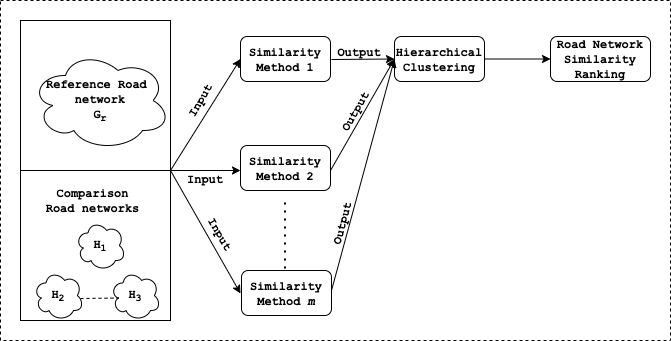
\includegraphics[width=1.25\textwidth,center]{picture/network_ranking.png}
\caption[Miniaturtrichter]{Road Networking Similarity and Ranking}
\label{fig:network ranking}
\end{figure}

\subsection{Grid Road Network Similarity Analysis}
\subsection{Radial Road Network Similarity Analysis}
\subsection{Tree Road Network Similarity Analysis}
\subsection{Linear Road Network Similarity Analysis}
\subsection{Cul de Sac Road Network Similarity Analysis}

    
\chapter{Conclusion}
    %%%%%%%%%%%%%%%
% Conclusion %
%%%%%%%%%%%%%%%

In summary, this was the first study to compare the performance of various graph-based similarity algorithms on two different road network data sets. Furthermore, each of the methods used was compared to one another in order to identify similarities.

The results of the similarity measure between the different road networks, as well as the correlations between each method used with the Kendall tau distance, varied depending on the type of road network used for the comparison. An intriguing discovery was that the clustering algorithm was able to identify clusters of road networks that have similar structures of the road networks as graphs, which goes slightly against the initial approach of identifying road networks with similar patterns such as Grid, Radial, Tree, Linear, or Cul De Sac as the algorithms themselves do not take the patterns of the road networks into consideration when comparing them but the topological characteristics which are stored in the graph structure.

A close examination of the dendrograms that identified clusters among the road networks, on the other hand, reveals that specific road networks with similar patterns belonged to the same cluster. The road networks of Champs-Elysees in Paris, Amsterdam, and the City of Westminster in London, for example, all belonged to the same cluster with shorter distances, as did Toronto-Canada, Ejecutivo-Mexico City, and the District of Columbia-USA. Because they operated at different levels and used different comparisons, each similarity measure behaved differently, as expected from the correlation to identify similarities in the similarity methods. Despite this, cosine similarity, Euclidean distance, Jaccard distance, and Jaccard similarity have strong correlations.


\section{Future Directions}
Because this research into identifying similarities on road networks as graphs is still in its early stages. From a methodological standpoint, more efforts should be made to conduct studies that compare alternative methods to those presented in section 3. Furthermore, the method for selecting road networks should be researched. Following that, a more in-depth examination of the study's findings is required to provide precise conclusions on the utility of similarity measures in this context, followed by more appropriate validation of the clustering results. Finally, more work is required to develop and optimize similarity algorithms that combine multiple graph properties into a single similarity score. Before applying these algorithms to real-world road networks, they should be tested and validated on simulated data (where ground truth can be obtained to some extent). Another methodological approach is to use similarity methods in dynamic road algorithms to decipher how road networks change over time. To compare adjacent networks, most dynamic analysis algorithms require a similarity/correlation step. The classical correlation coefficient is commonly used [\cite{ONeill:2018}]. The incorporation of a network-based similarity index into dynamic road algorithms can improve their performance significantly.
It is hoped that this study will inspire other researchers to contribute ideas in the field of road network similarity that are not described above, either methodologically or practically.

\chapter{Appendix}
%%%%%%%%%%%%
% Appendix %
%%%%%%%%%%%%



\printbibliography %Prints bibliography

\end{document}
